\chapter{Projeto do Serviço em Nuvem}\label{chp:serviconuvem}
Este capítulo possui a finalidade de projetar e implementar um serviço em nuvem acessível aos controladores locais da rede de sensores, de modo a alcançar o objetivo (ii) do trabalho. Os tópicos abordados neste capítulo englobam o protocolo de troca de dados envolvendo o servidor em nuvem (batizado de Homecloud), a interface de controle do usuário e a especificação de um algoritmo de aprendizagem específico para o domínio de controle de iluminação.

\section{O Protocolo Homecloud} \label{sec:homecloud}
Conforme mencionado na seção \ref{sec:arquitetura}, o servidor em nuvem se comunica tanto com o controlador local quanto com o dispositivo de interface do usuário. O protocolo Homecloud, definido pelo grupo, define o formato das mensagens a serem trocados pelos dispositivos, e em quais circunstâncias. As próximas seções especificarão em detalhes o funcionamento deste protocolo.

\subsection{Sintaxe e Semântica} \label{subsec:hc_sintaxe}
Para melhor organizar as mensagens do protocolo, elas serão agrupadas no decorrer deste relatório em quatro classes de acordo com a sua função, a saber:

\begin{itemize}
	\item Mensagens de Estado: Transmitem informações relativas ao estado da casa, incluindo dados lidos de sensores, estados de atuadores e ações tomadas pelo usuário;
	\item Mensagens de Regras: Referem-se à definição de regras de automação pelo usuário ou pelo sistema de aprendizagem de máquina;
	\item Mensagens de Gerenciamento dos Nós: Transmitem informações e comandos relativos aos nós (sensores e atuadores) da rede local;
	\item Mensagens de Autenticação: Responsáveis por carregar dados de autenticação dos agentes do sistema.
\end{itemize}

As mensagens são enviadas ao servidor através de requisições HTTP. Portanto, cada mensagem possui uma resposta de um determinado tipo, a depender da natureza das informações solicitadas.  Notificações destinadas aos usuários ou aos controladores não esperam resposta, pois são enviadas por meio protocolos que não seguem o modelo de requisição-resposta. 

A seguir serão definidas as mensagens, de acordo com a classificação apresentada, bem como as respectivas respostas esperadas. 

\subsubsection{Mensagens de Estado}
As mensagens de estado estão listadas e descritas na Tabela \ref{tab:mensagens_estado}. Nesta tabela, o sentido de tráfego das mensagens estão especificadas. Neste item, o termo ``aplicativo'' foi utilizado para se referir ao dispositivo utilizado pelo usuário para interagir com o sistema, que poderia ser um aplicativo em um \textit{smartphone}.

\begin{table}[h]
	\centering
	\caption{Listagem e descrição das Mensagens de Estado.}\smallskip
	\label{tab:mensagens_estado}
	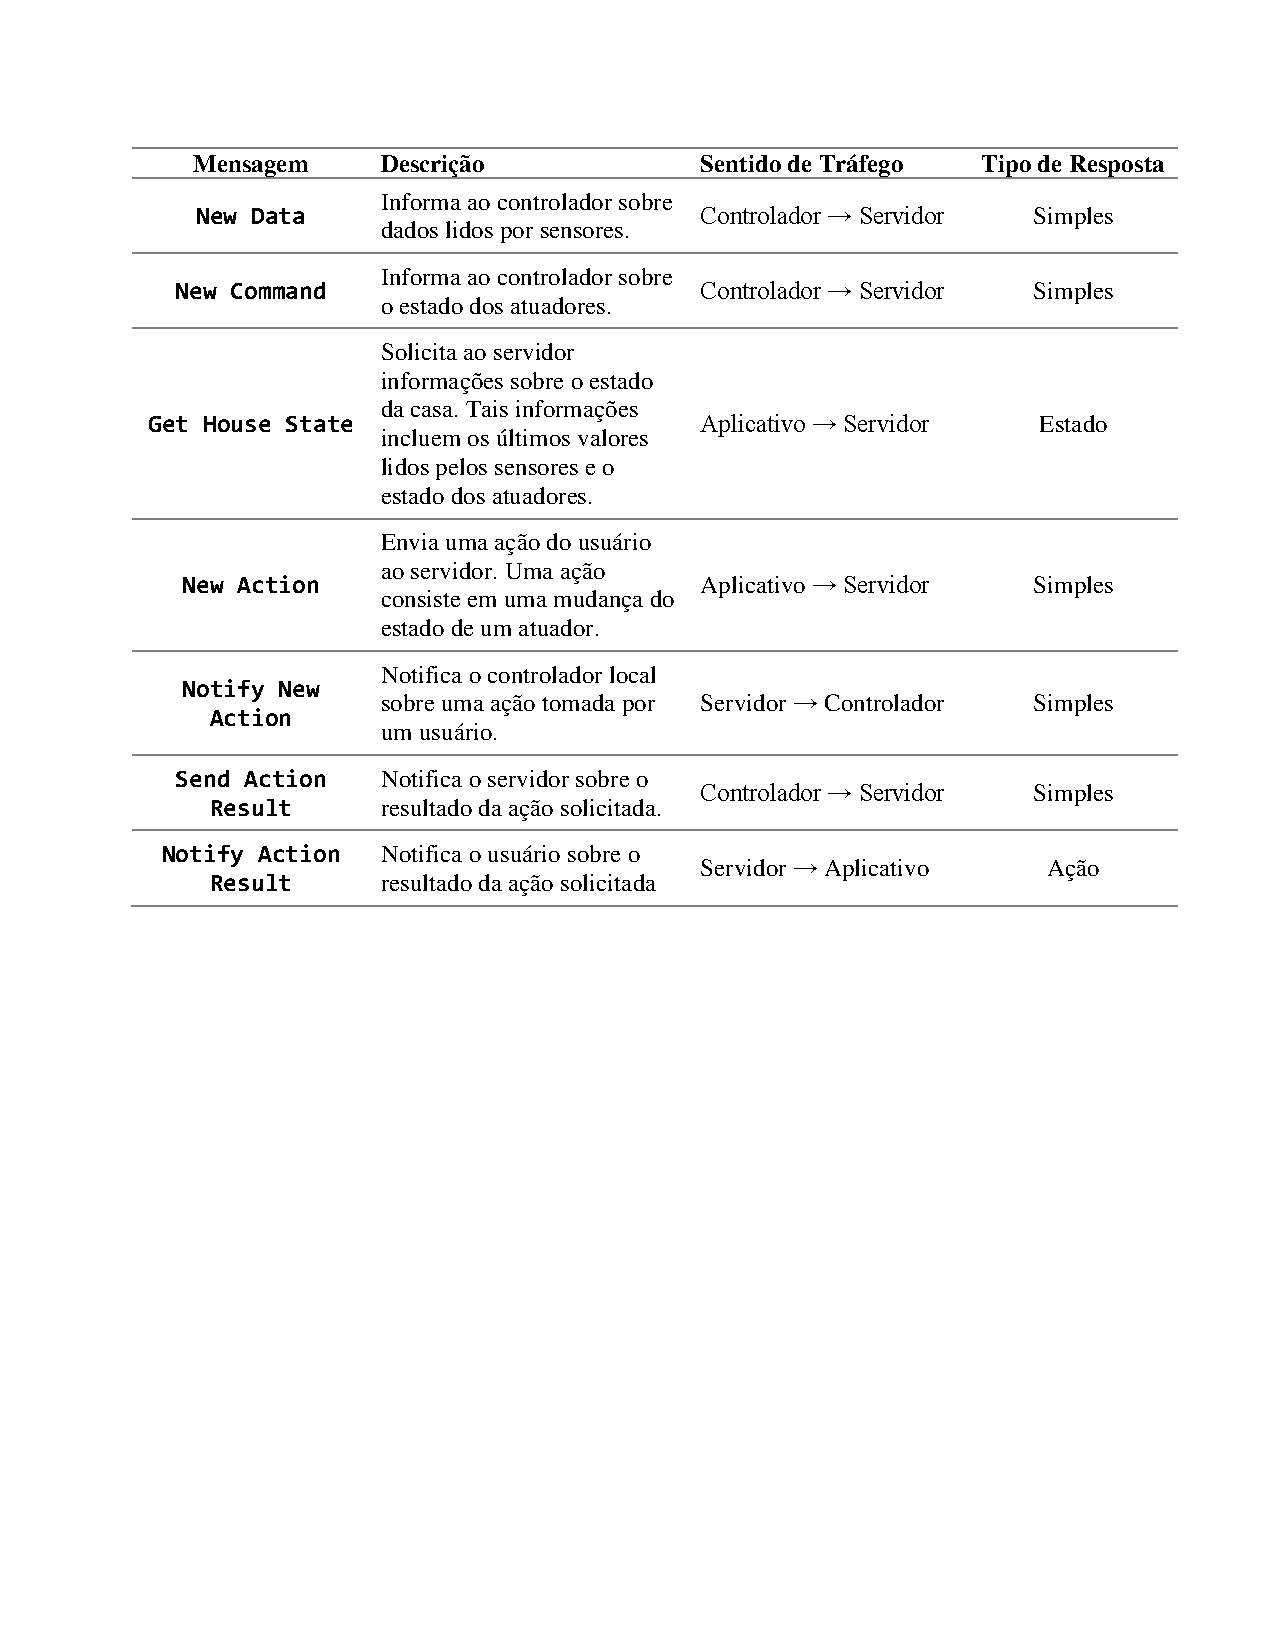
\includegraphics[width=\textwidth]{tabelas/mensagens_estado.pdf}
\end{table}

A seguir, será detalhado o conteúdo de cada mensagem listada na Tabela \ref{tab:mensagens_estado}. As mensagens seguem o formato JSON, e os campos com valor variável estão circundados pelos símbolos \texttt{< >}.

\paragraph*{\texttt{New Data}.} A Listagem \ref{lst:newData} ilustra o formato da mensagem. O campo \texttt{function} contém o nome da mensagem, a ser utilizado pelo servidor para efetuar o tratamento adequado. O campo \texttt{data} contém uma lista de objetos, cada qual representando uma leitura de um sensor.

\noindent
\begin{minipage}[l]{\linewidth}
\lstinputlisting[label=lst:newData, caption=Formato da mensagem \texttt{newData}.]{codigos/newData.json}
\end{minipage}

\paragraph*{\texttt{New Command}.} A Listagem \ref{lst:newCommand} ilustra o formato da mensagem. O campo \texttt{command} contém uma lista de objetos, cada qual representando uma estado de um atuador.

\noindent
\begin{minipage}[l]{\linewidth}
\lstinputlisting[label=lst:newCommand, caption=Formato da mensagem \texttt{newCommand}.]{codigos/newCommand.json}
\end{minipage}

\paragraph*{\texttt{Get House State}.} A Listagem \ref{lst:getHouseState} ilustra o formato da mensagem.

\noindent
\begin{minipage}[l]{\linewidth}
\lstinputlisting[label=lst:getHouseState, caption=Formato da mensagem \texttt{getHouseState}.]{codigos/getHouseState.json}
\end{minipage}

\paragraph*{\texttt{New Action}.} A Listagem \ref{lst:newAction} ilustra o formato da mensagem. O campo \texttt{action} contém um objeto que representa uma ação a ser tomada. Lembre-se de que uma ação é definida pelo estado de um comando de um atuador, que o usuário supostamente deseja alterar.

\noindent
\begin{minipage}[l]{\linewidth}
\lstinputlisting[label=lst:newAction, caption=Formato da mensagem \texttt{newAction}.]{codigos/newAction.json}
\end{minipage}

\paragraph*{\texttt{Notify New Action}.} A Listagem \ref{lst:notifyNewAction} ilustra o formato da mensagem. O campo \texttt{action} contém um objeto que representa uma ação a ser tomada. Note que as mensagens originadas do servidor e destinadas ao aplicativo ou ao controlador possuem um campo \texttt{notification} que lista o nome da mensagem, em contraste com as mensagens destinadas ao servidor.

\noindent
\begin{minipage}[l]{\linewidth}
\lstinputlisting[label=lst:notifyNewAction, caption=Formato da mensagem \texttt{notifyNewAction}.]{codigos/notifyNewAction.json}
\end{minipage}

\paragraph*{\texttt{Send Action Result}.} A Listagem \ref{lst:sendActionResult} ilustra o formato da mensagem. O campo \texttt{action} contém um objeto que representa a ação que o usuário solicitou. O campo \texttt{result} contém um valor booleano que indica se a ação solicitada foi efetuada com sucesso.

\noindent
\begin{minipage}{\linewidth}
\lstinputlisting[label=lst:sendActionResult, caption=Formato da mensagem \texttt{sendActionResult}.]{codigos/sendActionResult.json}
\end{minipage}

\paragraph*{\texttt{Notify Action Result}.} A Listagem \ref{lst:notifyActionResult} ilustra o formato da mensagem. O campo \texttt{action} contém um objeto que representa a ação que o usuário solicitou. O campo \texttt{result} contém um valor booleano que indica se a ação solicitada foi efetuada com sucesso.

\noindent
\begin{minipage}{\linewidth}
\lstinputlisting[label=lst:notifyActionResult, caption=Formato da mensagem \texttt{notifyActionResult}.]{codigos/notifyActionResult.json}
\end{minipage}

\subsubsection{Mensagens de Regra}
As mensagens de regra estão listadas e descritas na Tabela \ref{tab:mensagens_regra}.

\begin{table}[h]
	\centering
	\caption{Listagem e descrição das Mensagens de Regra.}\smallskip
	\label{tab:mensagens_regra}
	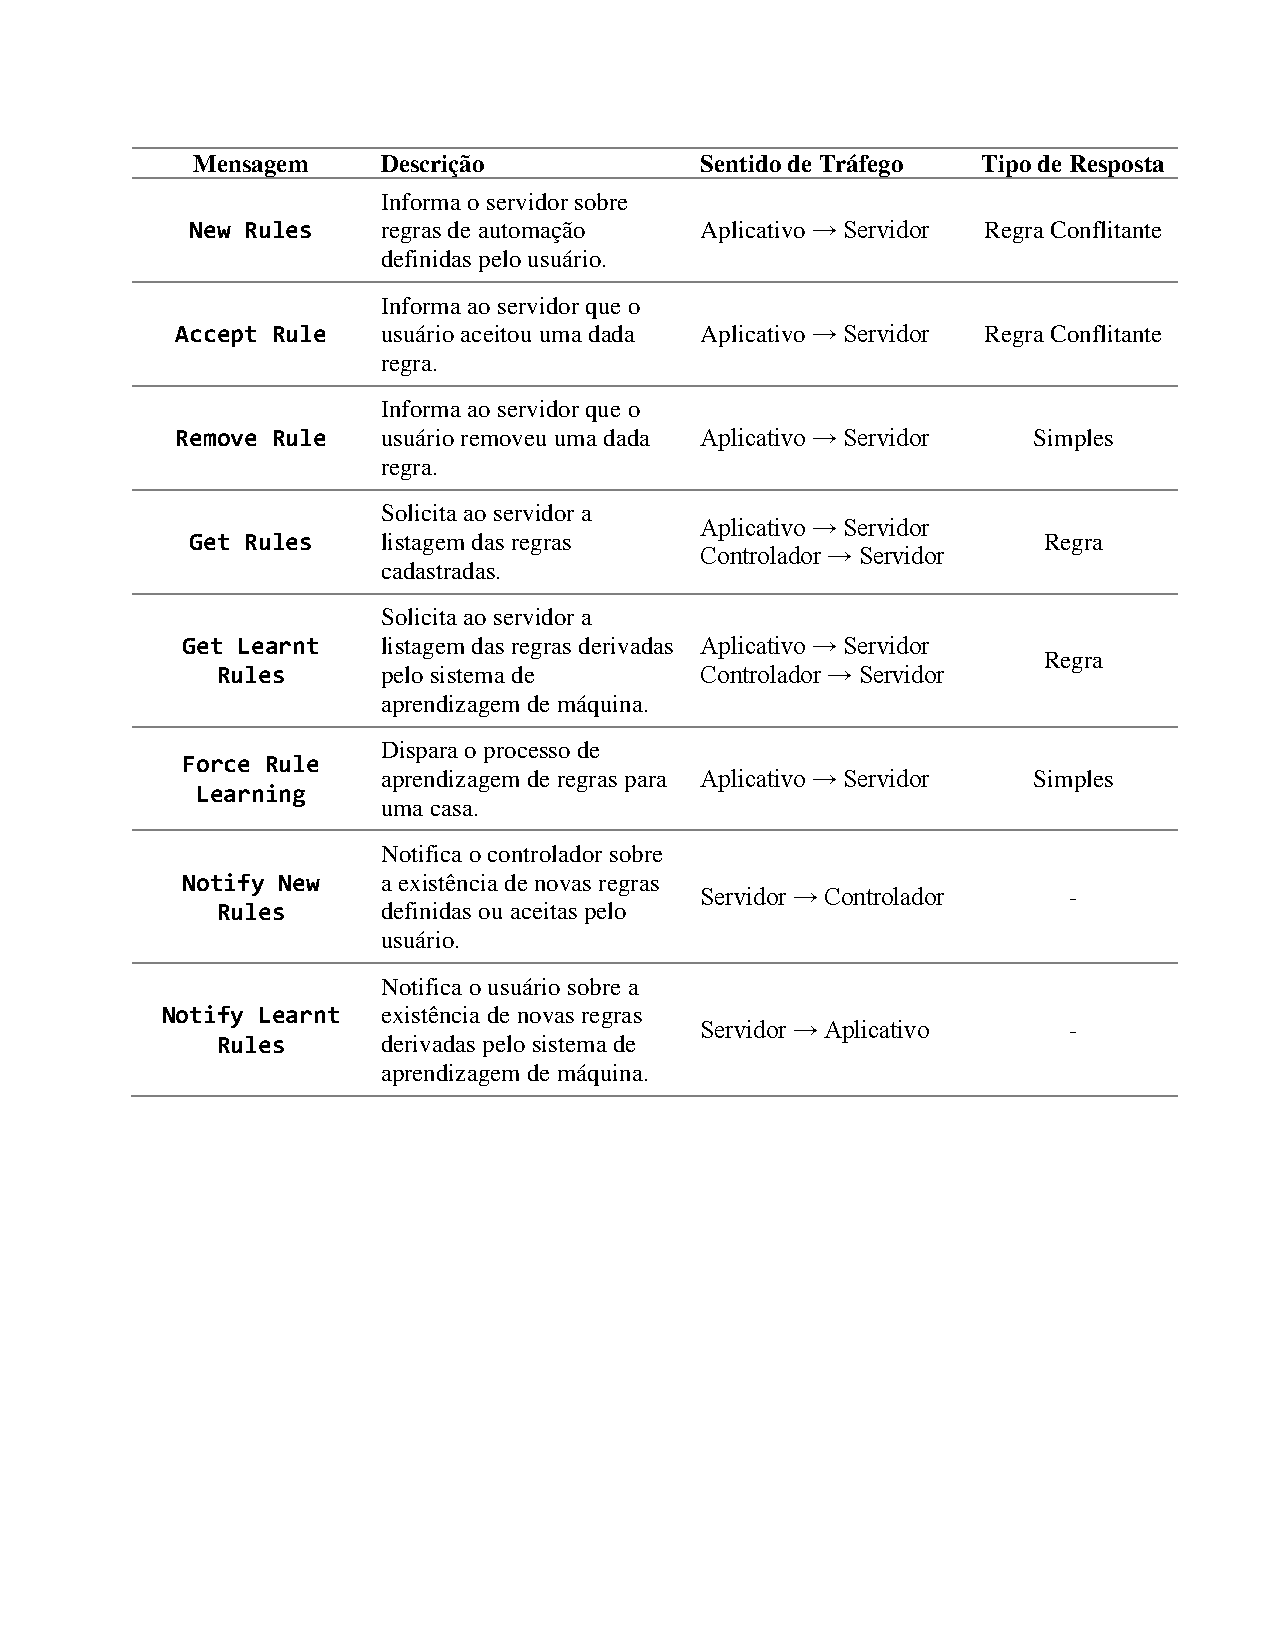
\includegraphics[width=\textwidth]{tabelas/mensagens_regra.pdf}
\end{table}

\paragraph*{\texttt{New Rules}.} A Listagem \ref{lst:newRules} ilustra o formato da mensagem. Uma mensagem deste tipo pode definir diversas regras, declaradas no campo \texttt{rules}. Cada regra especifica o nó-alvo(\texttt{nodeId}), o controlador associado (\texttt{controllerId}), o comando interno do nó (\texttt{commandId}) e o valor que este comando deve assumir (\texttt{value}) caso a condição representada pela cláusula (\texttt{clause}) se mostre verdadeira. Uma cláusula consiste em uma expressão booleana representada em DNF, codificada, na listagem, como uma lista de listas de proposições.

\noindent
\begin{minipage}[l]{\linewidth}
\lstinputlisting[label=lst:newRules, caption=Formato da mensagem \texttt{newRules}.]{codigos/newRules.json}
\end{minipage}

\paragraph*{\texttt{Accept Rule}.} A Listagem \ref{lst:acceptRule} ilustra o formato da mensagem. Esta mensagem indica a decisão do usuário em aceitar a regra explicitada no corpo da mensagem.

\noindent
\begin{minipage}[l]{\linewidth}
\lstinputlisting[label=lst:acceptRule, caption=Formato da mensagem \texttt{acceptRule}.]{codigos/acceptRule.json}
\end{minipage}

\paragraph*{\texttt{Remove Rule}.} A Listagem \ref{lst:removeRule} ilustra o formato da mensagem. Esta mensagem indica a decisão do usuário em remover uma regra já cadastrada no sistema (definida ou previamente aceita por ele).

\noindent
\begin{minipage}[l]{\linewidth}
\lstinputlisting[label=lst:removeRule, caption=Formato da mensagem \texttt{removeRule}.]{codigos/removeRule.json}
\end{minipage}

\paragraph*{\texttt{Get Rules}.} A Listagem \ref{lst:getRules} ilustra o formato da mensagem.

\noindent
\begin{minipage}[l]{\linewidth}
\lstinputlisting[label=lst:getRules, caption=Formato da mensagem \texttt{getRules}.]{codigos/getRules.json}
\end{minipage}

\paragraph*{\texttt{Get Learnt Rules}.} A Listagem \ref{lst:getLearntRules} ilustra o formato da mensagem.

\noindent
\begin{minipage}[l]{\linewidth}
\lstinputlisting[label=lst:getLearntRules, caption=Formato da mensagem \texttt{getLearntRules}.]{codigos/getLearntRules.json}
\end{minipage}

\paragraph*{\texttt{Force Rule Learning}.} A Listagem \ref{lst:forceRuleLearning} ilustra o formato da mensagem.

\noindent
\begin{minipage}[l]{\linewidth}
\lstinputlisting[label=lst:forceRuleLearning, caption=Formato da mensagem \texttt{forceRuleLearning}.]{codigos/forceRuleLearning.json}
\end{minipage}

\paragraph*{\texttt{Notify New Rules}.} A Listagem \ref{lst:notifyNewRules} ilustra o formato da mensagem. O campo \texttt{quantity} contém o número de novas regras disponíveis para adicionar ao banco de dados do controlador.

\noindent
\begin{minipage}[l]{\linewidth}
\lstinputlisting[label=lst:notifyNewRules, caption=Formato da mensagem \texttt{notifyNewRules}.]{codigos/notifyNewRules.json}
\end{minipage}

\paragraph*{\texttt{Notify Learnt Rules}.} A Listagem \ref{lst:notifyLearntRules} ilustra o formato da mensagem. O campo \texttt{quantity} contém o número de novas regras disponíveis para análise do usuário.

\noindent
\begin{minipage}[l]{\linewidth}
\lstinputlisting[label=lst:notifyLearntRules, caption=Formato da mensagem \texttt{notifyLearntRules}.]{codigos/notifyLearntRules.json}
\end{minipage}

\subsubsection{Mensagens de Gerenciamento de Nós}
As mensagens de gerenciamento de nós estão listadas e descritas na Tabela \ref{tab:mensagens_nos}.

\begin{table}[hp]
	\centering
	\caption{Listagem e descrição das Mensagens de Gerenciamento de Nós.}\smallskip
	\label{tab:mensagens_nos}
	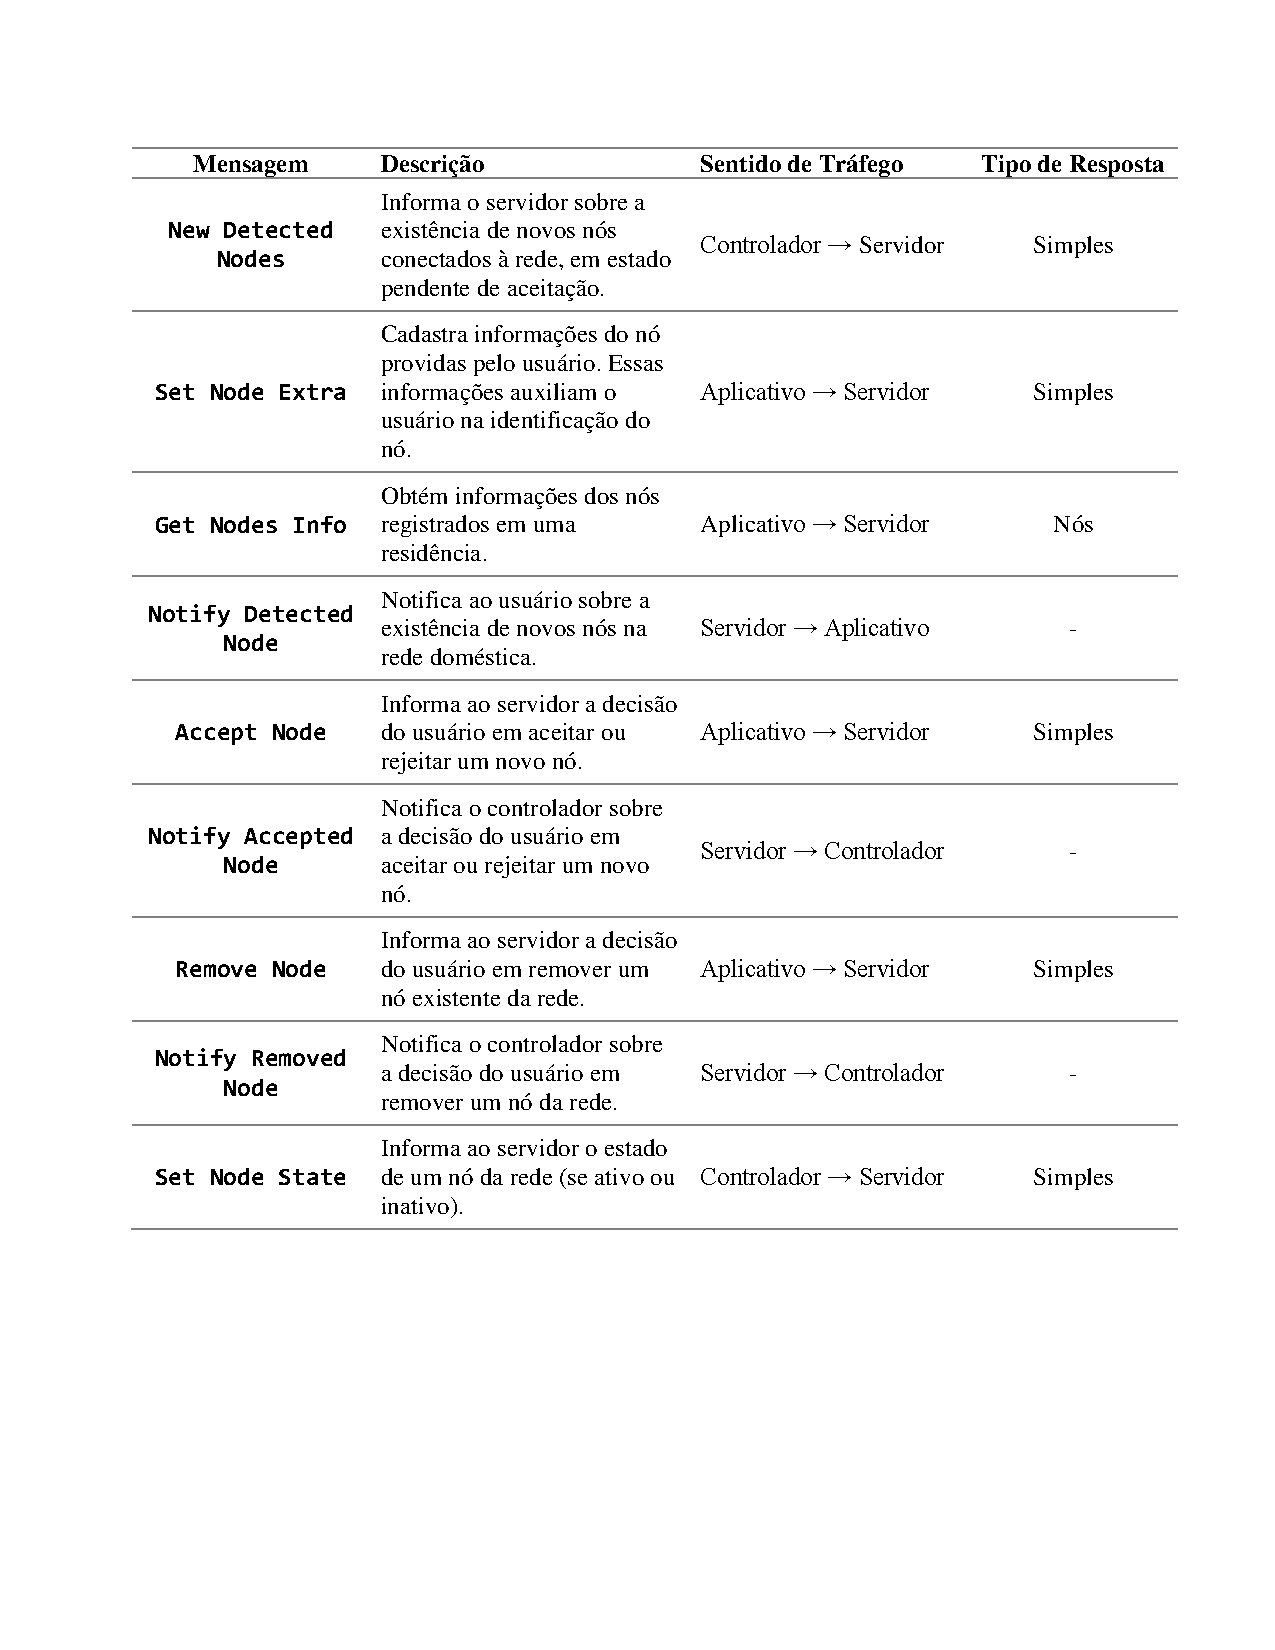
\includegraphics[width=\textwidth]{tabelas/mensagens_nos.pdf}
\end{table}

\paragraph*{\texttt{New Detected Nodes}.} A Listagem \ref{lst:newDetectedNodes} ilustra o formato da mensagem. O campo \texttt{node} contém informações utilizadas na descrição do nó, e reflete os campos utilizados nas mensagens de \texttt{description} do protocolo \textit{Rainfall}, definido na \ref{subsec:sintaxe}. Por exemplo, estão presentes na mensagem o identificador do nó (\texttt{nodeId}), sua classe (\texttt{nodeClass}), informações dos dados lidos pelo nó (\texttt{dataType}) bem como dos comandos aceitos por ele (\texttt{commandType}).

\noindent
\begin{minipage}[l]{\linewidth}
\lstinputlisting[label=lst:newDetectedNodes, caption=Formato da mensagem \texttt{newDetectedNodes}.]{codigos/newDetectedNodes.json}
\end{minipage}

\paragraph*{\texttt{Set Node Extra}.} A Listagem \ref{lst:setNodeExtra} ilustra o formato da mensagem. Os campos \texttt{nodeId} e \texttt{controllerId} definem o nó para o qual se deseja definir informações extras. O campo \texttt{extra}, por sua vez, contém as informações propriamente ditas. Por exemplo, o mapeamento poderia incluir uma chave ``Nome'' com valor ``Interruptor de luz'', atribuindo, assim, um nome a um dado nó da casa.

\noindent
\begin{minipage}[l]{\linewidth}
\lstinputlisting[label=lst:setNodeExtra, caption=Formato da mensagem \texttt{setNodeExtra}.]{codigos/setNodeExtra.json}
\end{minipage}

\paragraph*{\texttt{Get Nodes Info}.} A Listagem \ref{lst:getNodesInfo} ilustra o formato da mensagem.

\noindent
\begin{minipage}[l]{\linewidth}
\lstinputlisting[label=lst:getNodesInfo, caption=Formato da mensagem \texttt{getNodesInfo}.]{codigos/getNodesInfo.json}
\end{minipage}

\paragraph*{\texttt{Notify Detected Nodes}.} A Listagem \ref{lst:notifyDetectedNode} ilustra o formato da mensagem. O campo \texttt{quantity} contém a quantidade de novos nós na rede.

\noindent
\begin{minipage}[l]{\linewidth}
\lstinputlisting[label=lst:notifyDetectedNode, caption=Formato da mensagem \texttt{notifyDetectedNode}.]{codigos/notifyDetectedNode.json}
\end{minipage}

\paragraph*{\texttt{Accept Node}.} A Listagem \ref{lst:acceptNode} ilustra o formato da mensagem. Os campos \texttt{nodeId} e \texttt{controllerId} identificam o nó que será aceito ou rejeitado, a depender do valor do campo \texttt{accept}.

\noindent
\begin{minipage}[l]{\linewidth}
\lstinputlisting[label=lst:acceptNode, caption=Formato da mensagem \texttt{acceptNode}.]{codigos/acceptNode.json}
\end{minipage}

\paragraph*{\texttt{Notify Accepted Node}.} A Listagem \ref{lst:notifyAcceptedNode} ilustra o formato da mensagem. O campo \texttt{nodeId} identifica o nó que será aceito ou rejeitado, a depender do valor do campo \texttt{accept}.

\noindent
\begin{minipage}[l]{\linewidth}
\lstinputlisting[label=lst:notifyAcceptedNode, caption=Formato da mensagem \texttt{notifyAcceptedNode}.]{codigos/notifyAcceptedNode.json}
\end{minipage}

\paragraph*{\texttt{Remove Node}.} A Listagem \ref{lst:removeNode} ilustra o formato da mensagem. Os campos \texttt{nodeId} e \texttt{controllerId} identificam o nó que será removido.

\noindent
\begin{minipage}[l]{\linewidth}
\lstinputlisting[label=lst:removeNode, caption=Formato da mensagem \texttt{removeNode}.]{codigos/removeNode.json}
\end{minipage}

\paragraph*{\texttt{Notify Removed Node}.} A Listagem \ref{lst:notifyRemovedNode} ilustra o formato da mensagem. O campo \texttt{nodeId} identifica o nó que será removido.

\noindent
\begin{minipage}[l]{\linewidth}
\lstinputlisting[label=lst:notifyRemovedNode, caption=Formato da mensagem \texttt{notifyRemovedNode}.]{codigos/notifyRemovedNode.json}
\end{minipage}

\paragraph*{\texttt{Set Node State}.} A Listagem \ref{lst:setNodeState} ilustra o formato da mensagem. O campo \texttt{nodeId} identifica o nó a que a mensagem se refere, ao passo que o campo \texttt{alive} indica se o nó está ativo (1) ou não (0).

\noindent
\begin{minipage}[l]{\linewidth}
\lstinputlisting[label=lst:setNodeState, caption=Formato da mensagem \texttt{setNodeState}.]{codigos/setNodeState.json}
\end{minipage}

\subsubsection{Mensagens de Autenticação}
O módulo de autenticação do sistema define uma série de mensagens para efetuar tarefas tais como identificação dos agentes do sistema, autorização de acesso e manutenção do banco de dados de agentes. Antes de apresentar as mensagens, cabe definir a terminologia utilizada neste tópico.
\begin{itemize}
	\item \textbf{Agente}: Qualquer entidade externa ao servidor que necessita de credenciais para se autenticar com ele. Pode ser um controlador local, um administrador ou um usuário;
	\item \textbf{Casa}: Neste documento, uma casa é essencialmente um agrupamento de agentes. Tipicamente, uma casa possui um ou mais controladores associados, um  administrador e diversos usuários.
	\item \textbf{Administrador}: Um agente que possui privilégios elevados para gerenciar uma casa, podendo associar controladores, adicionar usuários e aceitar ou remover nós da rede local. Cada casa possui um único administrador, e cada administrador é associado a apenas uma casa.
	\item \textbf{Usuário}: O administrador pode adicionar a uma casa agentes com privilégios reduzidos, denominados usuários. Os usuários podem acessar o estado da casa, definir regras e enviar comandos. Cada casa pode ter múltiplos usuários, e cada usuário pode estar associado a somente uma casa.
\end{itemize}

As mensagens de autenticação estão listadas e descritas na Tabela \ref{tab:mensagens_auth}.

\begin{table}[h]
	\centering
	\caption{Listagem e descrição das Mensagens de Autenticação.}\smallskip
	\label{tab:mensagens_auth}
	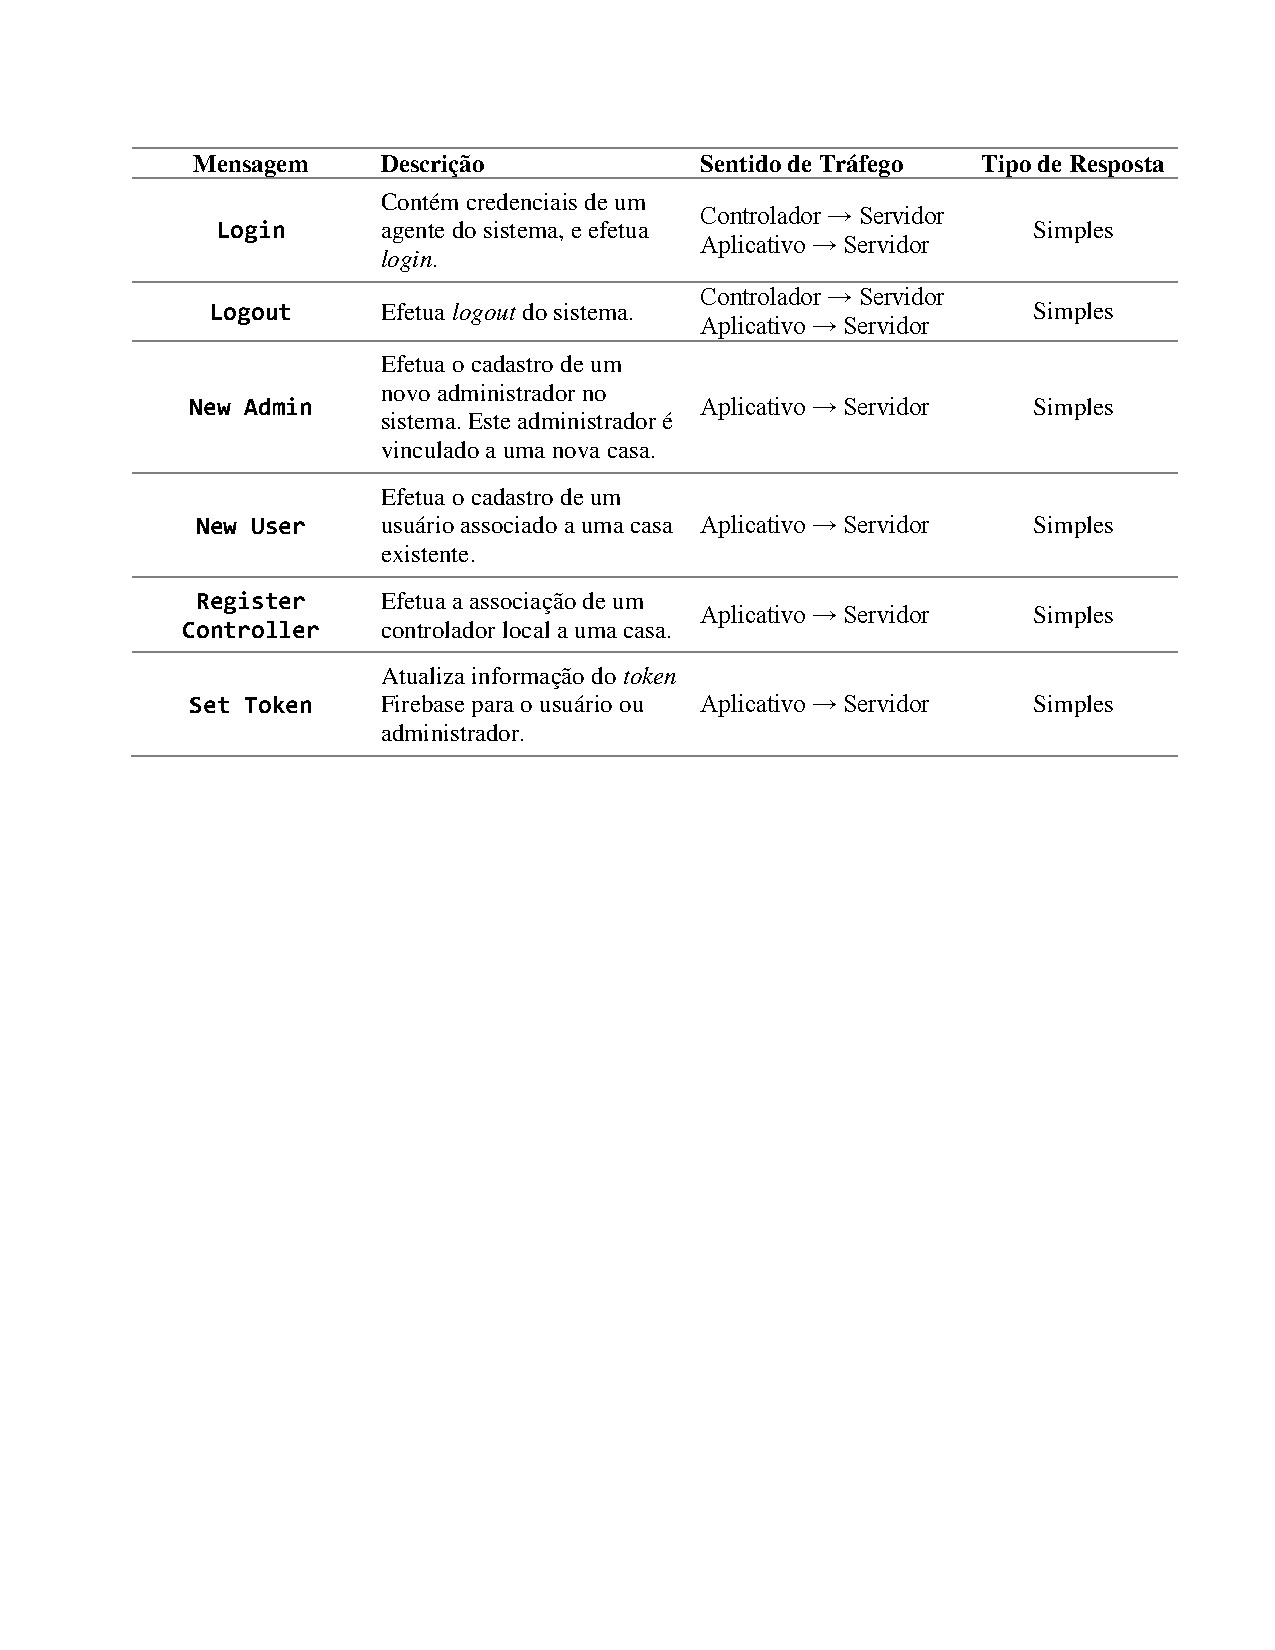
\includegraphics[width=\textwidth]{tabelas/mensagens_auth.pdf}
\end{table}

\paragraph*{\texttt{Login}.} A Listagem \ref{lst:login} ilustra o formato da mensagem. Os campos \texttt{username} e \texttt{password} contêm as credenciais do agente para fins de autenticação. O campo \texttt{token} é utilizado para informar ao servidor o código a ser utilizado para identificar o dispositivo a partir do qual a comunicação está sendo realizada, para de envio de notificação.

\noindent
\begin{minipage}[l]{\linewidth}
\lstinputlisting[label=lst:login, caption=Formato da mensagem \texttt{login}.]{codigos/login.json}
\end{minipage}

\paragraph*{\texttt{Logout}.} A Listagem \ref{lst:logout} ilustra o formato da mensagem. 

\noindent
\begin{minipage}[l]{\linewidth}
\lstinputlisting[label=lst:logout, caption=Formato da mensagem \texttt{logout}.]{codigos/logout.json}
\end{minipage}

\paragraph*{\texttt{New Admin}.} A Listagem \ref{lst:newAdmin} ilustra o formato da mensagem. Os campos \texttt{username} e \texttt{password} contêm as credenciais do administrador a ser cadastrado.

\noindent
\begin{minipage}[l]{\linewidth}
\lstinputlisting[label=lst:newAdmin, caption=Formato da mensagem \texttt{newAdmin}.]{codigos/newAdmin.json}
\end{minipage}

\paragraph*{\texttt{New User}.} A Listagem \ref{lst:newUser} ilustra o formato da mensagem. Os campos \texttt{username} e \texttt{password} contêm as credenciais do usuário a ser cadastrado. O servidor associa o novo usuário à mesma casa do agente que efetuou o cadastramento.

\noindent
\begin{minipage}[l]{\linewidth}
\lstinputlisting[label=lst:newUser, caption=Formato da mensagem \texttt{newUser}.]{codigos/newUser.json}
\end{minipage}

\paragraph*{\texttt{Register Controller}.} A Listagem \ref{lst:registerController} ilustra o formato da mensagem. O campo \texttt{controllerId} contém o identificador do controlador a ser associado à casa. Este controlador deve estar pré-cadastrado no banco de dados do servidor.

\noindent
\begin{minipage}[l]{\linewidth}
\lstinputlisting[label=lst:registerController, caption=Formato da mensagem \texttt{registerController}.]{codigos/registerController.json}
\end{minipage}

\paragraph*{\texttt{Set Token}.} A Listagem \ref{lst:setToken} ilustra o formato da mensagem. O campo \texttt{killToken} contém o \textit{token} antigo a ser substituído, ao passo que o campo \texttt{token} contém o novo \textit{token}. 

\noindent
\begin{minipage}[l]{\linewidth}
\lstinputlisting[label=lst:setToken, caption=Formato da mensagem \texttt{setToken}.]{codigos/setToken.json}
\end{minipage}

\paragraph*{\texttt{Get Controllers}.} A Listagem \ref{lst:getControllers} ilustra o formato da mensagem.

\noindent
\begin{minipage}[l]{\linewidth}
\lstinputlisting[label=lst:getControllers, caption=Formato da mensagem \texttt{getControllers}.]{codigos/getControllers.json}
\end{minipage}

\paragraph*{\texttt{Get Users}.} A Listagem \ref{lst:getUsers} ilustra o formato da mensagem.

\noindent
\begin{minipage}[l]{\linewidth}
\lstinputlisting[label=lst:getUsers, caption=Formato da mensagem \texttt{getUsers}.]{codigos/getUsers.json}
\end{minipage}

\subsubsection{Mensagens de Resposta}
Conforme apresentado nas Tabelas \ref{tab:mensagens_estado}, \ref{tab:mensagens_regra}, \ref{tab:mensagens_nos} e \ref{tab:mensagens_auth}, cada mensagem destinada ao servidor espera uma mensagem de uma determinada classe, a depender da natureza da requisição. Nesta seção, o formato dessas mensagens de resposta será detalhado.

\paragraph*{Resposta Simples.} O formato desta resposta está ilustrado na Listagem \ref{lst:simpleResponse}. A resposta simples possui somente dois campos, presentes em todos os tipos de resposta: \texttt{status}, com um código representando o resultado da requisição (a numeração possui a mesma semântica da encontrada nas respostas HTTP), e \texttt{errorMessage}, contendo uma mensagem de erro caso existente.

\noindent
\begin{minipage}[l]{\linewidth}
\lstinputlisting[label=lst:simpleResponse, caption=Formato de uma Resposta Simples. ]{codigos/simpleResponse.json}
\end{minipage}

\paragraph*{Resposta de Estado.} O formato desta resposta está ilustrado na Listagem \ref{lst:simpleResponse}. A resposta de estado possui um campo além dos presentes na Resposta Simples, chamado \texttt{state}. Este campo possui informações dos últimos dados lidos pelo dispositivo, caso seja sensor, e dos estados dos comandos suportados, caso seja atuador.

\noindent
\begin{minipage}[l]{\linewidth}
\lstinputlisting[label=lst:stateResponse, caption=Formato de uma Resposta Simples. ]{codigos/stateResponse.json}
\end{minipage}

\paragraph*{Resposta de Regra Conflitante.} O formato desta resposta está ilustrado na Listagem \ref{lst:confRuleResponse}. Esta resposta possui um campo \texttt{conflictingRule} que especifica se uma regra definida ou aceita pelo usuário conflita com uma regra já existente no sistema.

\noindent
\begin{minipage}[l]{\linewidth}
\lstinputlisting[label=lst:confRuleResponse, caption=Formato de uma Resposta de Regra Conflitante. ]{codigos/confRuleResponse.json}
\end{minipage}

\paragraph*{Resposta de Regras.} O formato desta resposta está ilustrado na Listagem \ref{lst:ruleResponse}. Esta resposta possui um campo \texttt{rule} que lista todas as regras que satisfazem a requisição enviada.

\noindent
\begin{minipage}[l]{\linewidth}
\lstinputlisting[label=lst:ruleResponse, caption=Formato de uma Resposta de Regras. ]{codigos/ruleResponse.json}
\end{minipage}

\paragraph*{Resposta de Controladores.} O formato desta resposta está ilustrado na Listagem \ref{lst:controllerResponse}. Esta resposta possui um campo \texttt{controllers} que lista todos os controladores associados ao usuário que efetuou a requisição.

\noindent
\begin{minipage}[l]{\linewidth}
\lstinputlisting[label=lst:controllerResponse, caption=Formato de uma Resposta de Controladores.]{codigos/controllerResponse.json}
\end{minipage}

\paragraph*{Resposta de Usuários.} O formato desta resposta está ilustrado na Listagem \ref{lst:usersResponse}. Esta resposta possui um campo \texttt{users} que lista todos os usuários associados ao administrador que efetuou a requisição.

\noindent
\begin{minipage}[l]{\linewidth}
\lstinputlisting[label=lst:usersResponse, caption=Formato de uma Resposta de Usuários.]{codigos/usersResponse.json}
\end{minipage}

\paragraph*{Resposta de Nós.} O formato desta resposta está ilustrado na Listagem \ref{lst:nodeResponse}. Esta resposta possui um campo \texttt{nodes} que lista todas os nós instalados em uma casa.

\lstinputlisting[label=lst:nodeResponse, caption=Formato de uma Resposta de Nós.,float=h]{codigos/nodeResponse.json}

\clearpage

\subsection{Protocolo de Troca de Mensagens}
Uma vez definidas as mensagens a serem trocadas, pode-se abordar a sequência esperada de troca de mensagens para os cenários de uso do protocolo. A maioria das mensagens definidas possui uma dinâmica de troca de mensagens simples:

\begin{itemize}
	\item Mensagens destinadas ao controlador ou ao servidor não esperam resposta, como mencionado no início da seção \ref{subsec:hc_sintaxe}, devido ao protocolo utilizado. As trocas de mensagens se assemelham ao mostrado no diagrama à esquerda da Figura \ref{fig:mensagens_simples}.
	\item Grande parte das mensagens destinadas ao servidor se resumem a um ciclo de requisição-resposta, como ilustrado no diagrama à direita da Figura \ref{fig:mensagens_simples}. Um exemplo deste caso é a mensagem \texttt{Get Nodes Info}, que recebe uma resposta do tipo ``Nós'' (ver Tabela \ref{tab:mensagens_nos}). O ciclo de troca de mensagens seria, então, o envio de uma mensagem \texttt{Get Nodes Info} ao servidor, seguido de uma Resposta de Nós.
\end{itemize}

\begin{figure}[h]
	\centering
	\caption{Sequências de trocas de mensagens em casos simples: notificações destinadas ao aplicativo ou ao controlador (esq.), e requisições destinadas ao servidor (dir.)}
  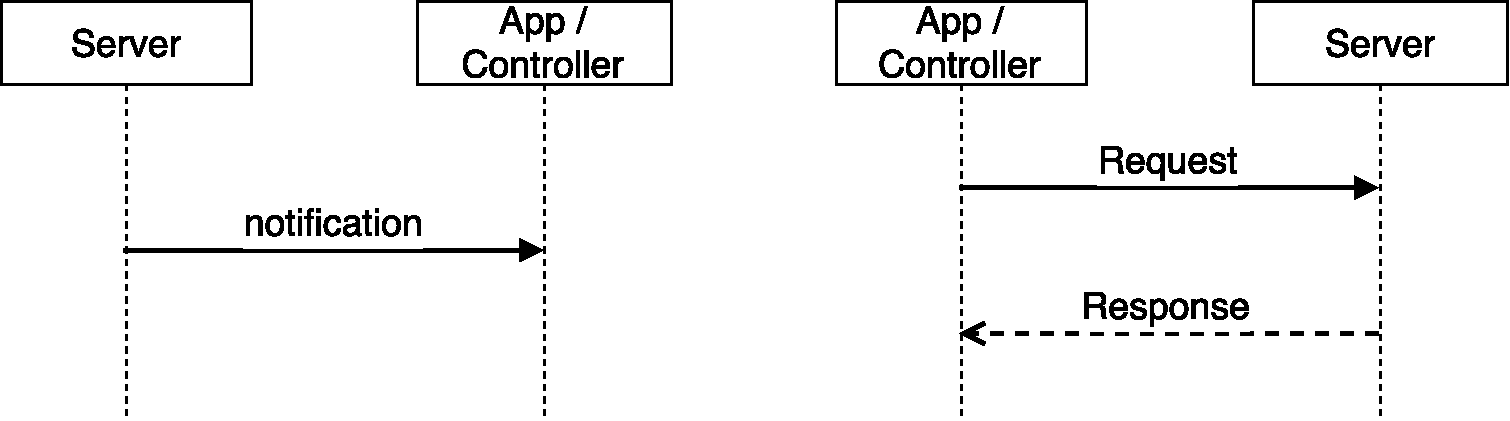
\includegraphics[width=\textwidth]{imagens/mensagens_simples.pdf}
  \label{fig:mensagens_simples}  
\end{figure}

A seguir, serão descritos alguns casos mais complexos de troca de mensagens, envolvendo múltiplas requisições e respostas definidos nas seções anteriores.

\paragraph*{Definição de uma Ação.}
A definição de uma ação pelo usuário envolve a utilização de diversas mensagens, como mostra a Figura \ref{fig:mensagens_new_action}. O ciclo se inicia com uma mensagem \texttt{New Action} do usuário (aplicativo) ao servidor. Conforme definido na Tabela \ref{tab:mensagens_estado}, uma mensagem deste tipo espera uma Resposta Simples. Em seguida, o servidor notifica o controlador através de uma mensagem \texttt{Notify New Action}, não recebendo resposta. Este, então, envia o resultado através de uma mensagem \texttt{Send Action Result}, recebendo uma Resposta Simples como resposta. Por fim, o servidor notifica o usuário através de uma mensagem \texttt{Notify Action Result}, não recebendo resposta.

\begin{figure}[h]
	\centering
	\caption{Sequência de trocas de mensagens na definição de uma nova ação.}
  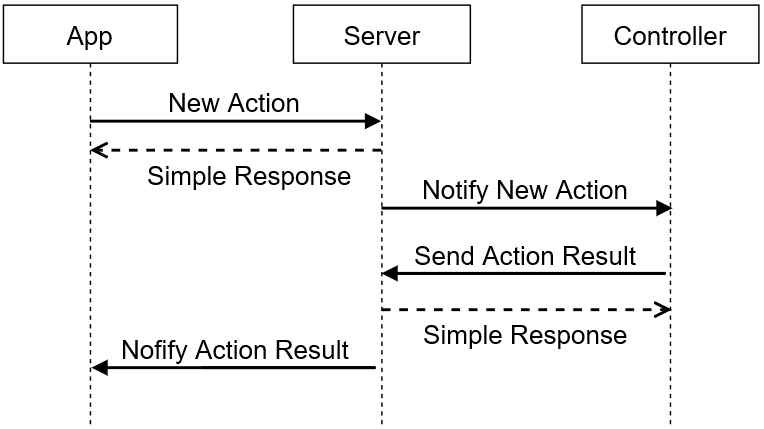
\includegraphics[width=0.7\textwidth]{imagens/mensagens_new_action.png}
  \label{fig:mensagens_new_action}  
\end{figure}

\paragraph*{Aceitação/Rejeição de um Nó.}
A Figura \ref{fig:mensagens_accept_node} mostra as mensagens trocadas neste processo. O controlador inicia enviando uma mensagem \texttt{Notify Detected Nodes} informando o servidor sobre a existência de novos nós. Este, por sua vez, informa ao usuário (aplicativo) que existe um novo nó com aceitação pendente através da mensagem \texttt{Notify Detected Node}. O usuário, então, responde com uma mensagem \texttt{Accept Node}, informando sua decisão ao servidor. Ele, por fim, envia uma notificação \texttt{Notify Accepted Node} ao controlador, informando-o da decisão do usuário.

\begin{figure}[h]
	\centering
	\caption{Sequência de trocas de mensagens na aceitação ou rejeição de um nó.}
  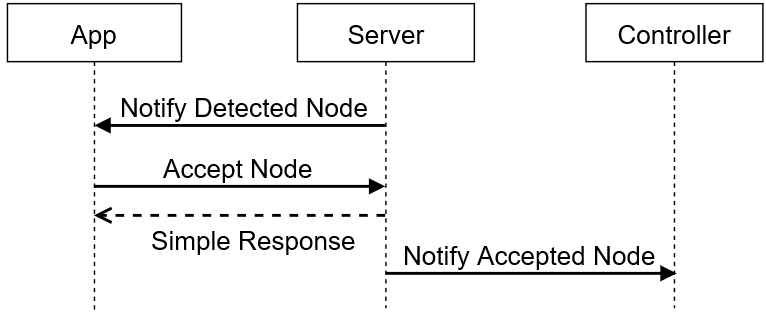
\includegraphics[width=0.7\textwidth]{imagens/mensagens_accept_node.png}
  \label{fig:mensagens_accept_node}  
\end{figure}

\paragraph*{Definição de Novas Regras.}
A Figura \ref{fig:mensagens_accept_rule} mostra as mensagens trocadas neste processo. O servidor inicia informando ao usuário (aplicativo) que existem novas regras para análise através da mensagem \texttt{Notify Learnt Rules}. O usuário, então, envia uma mensagem \texttt{Get Rules}, para que o servidor lhe envie as regras aprendidas através da Resposta de Regras. Após analisá-las, o usuário envia as regras aceitas na mensagem \texttt{Accept Rule} ao servidor. Este, por fim, envia uma notificação \texttt{Notify New Rules} ao controlador, informando-o sobre as novas regras.

\begin{figure}[h]
	\centering
	\caption{Sequência de trocas de mensagens na aceitação ou rejeição de um nó.}
  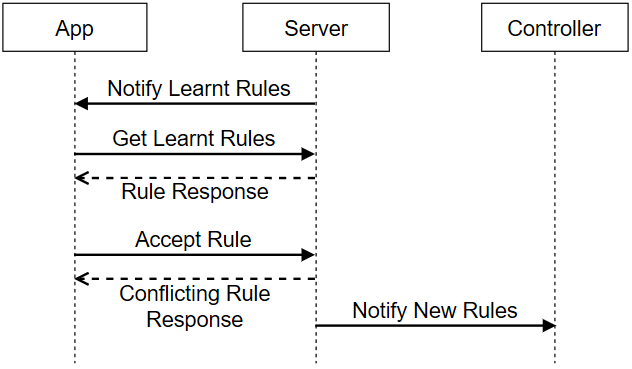
\includegraphics[width=0.7\textwidth]{imagens/mensagens_accept_rule.png}
  \label{fig:mensagens_accept_rule}  
\end{figure}

\section{Implementação do Protocolo Homecloud}
Conforme explicado na seção \ref{sec:homecloud}, o servidor, controlador e aplicativo devem todos oferecer suporte às mensagens do protocolo Homecloud que lhes dizem respeito. Para tanto, o grupo desenvolveu bibliotecas modulares para serem executadas nos três componentes. Antes de detalhar o processo de implementação de cada componente, cabe reapresentar a arquitetura geral do sistema, com ênfase nas tecnologias de comunicação utilizadas.

\subsection{Tecnologias de Comunicação Adotadas}
A Figura \ref{fig:arquitetura_tecnologias} ilustra a arquitetura do sistema com as tecnologias de comunicação utilizadas na comunicação entre cada uma de suas partes.

\begin{figure}[h]
	\centering
	\caption{Arquitetura do sistema com ênfase nas tecnologias de comunicação adotadas.}
  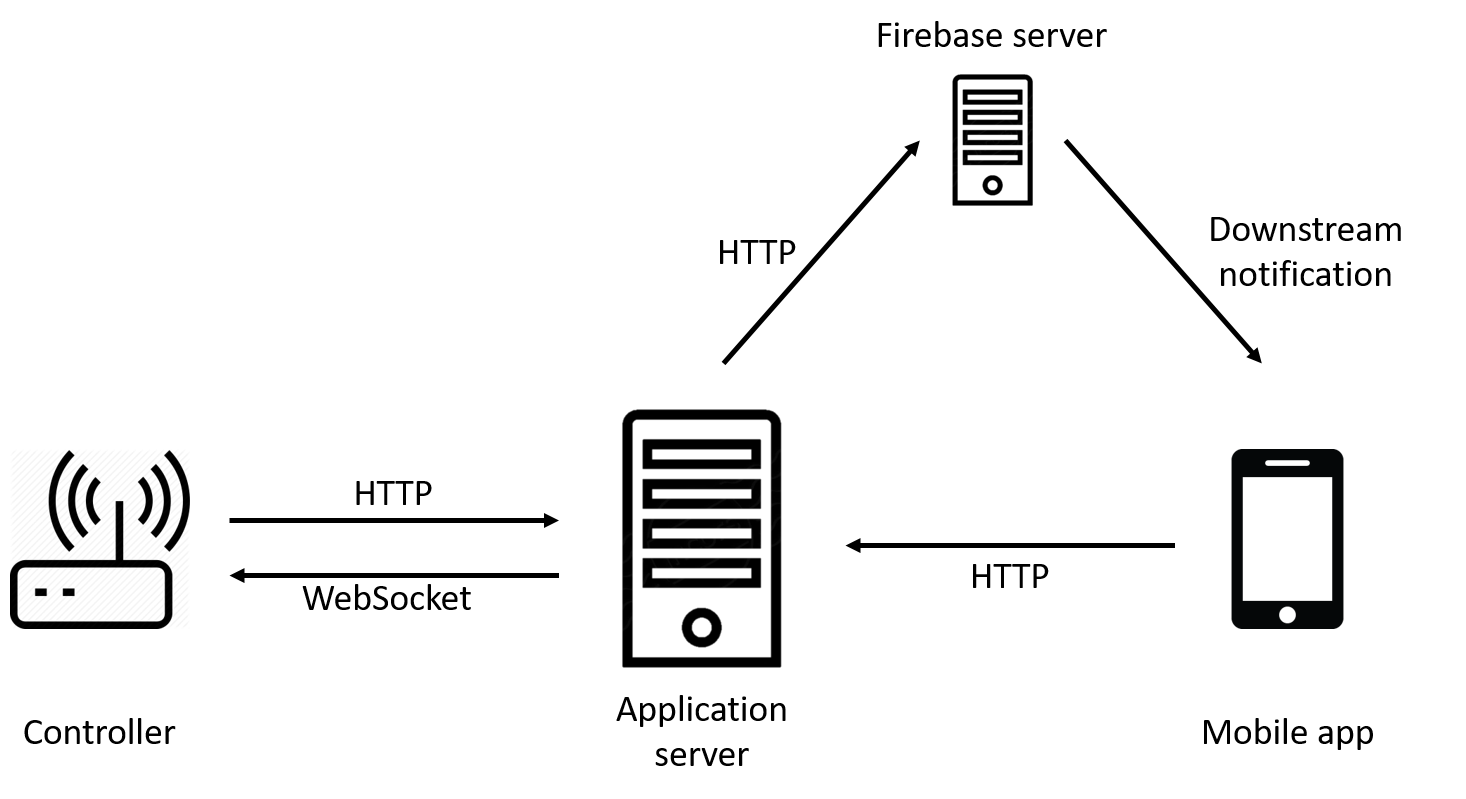
\includegraphics[width=0.7\textwidth]{imagens/arquitetura_tecnologias.png}
  \label{fig:arquitetura_tecnologias}  
\end{figure}

O primeiro ponto a destacar na arquitetura é o fato de toda a comunicação direcionada ao servidor ser feita através do protocolo HTTP. Essa escolha foi conveniente porque diversas mensagens do Homecloud exigem algum tipo de resposta (por exemplo, as mensagens \texttt{Get House State} e \texttt{Get Nodes Info}), e a natureza de requisição-resposta do HTTP supriu perfeitamente as necessidades do grupo. Soma-se a isso o fato de o HTTP ser amplamente adotado, possuindo bibliotecas nativas nas plataformas utilizadas para implementar os componentes do sistema.

Na seção \ref{subsec:hc_sintaxe}, foi apontado que mensagens destinadas ao controlador e ao aplicativo não esperavam resposta, devido ao protocolo de comunicação subjacente. Da Figura \ref{fig:arquitetura_tecnologias}, nota-se que a comunicação do servidor ao controlador é feito por meio do protocolo WebSocket \cite{rfc6455}, que não funciona no modo requisição-resposta como o HTTP.

A adoção deste protocolo nas comunicações do servidor ao controlador foi feita por satisfazer dois requisitos essenciais:
\begin{itemize}
	\item O protocolo deve permitir que um canal de comunicação persistente e confiável do servidor ao controlador seja aberto no momento em que o controlador se autentica com o servidor. Isso permite o envio de notificações ao controlador em tempo real;
	\item O protocolo deve ser padronizado, possuindo implementações disponíveis nas plataformas utilizadas para implementar o controlador e o servidor.
\end{itemize}

O protocolo WebSocket satisfaz aos dois requisitos mencionados. Em primeiro lugar, ele permite o estabelecimento de um canal \textit{full-duplex} entre as partes envolvidas sobre um canal TCP. Em segundo, ele é um padrão IETF definido com base no protocolo HTTP, possuindo diversas bibliotecas nas plataformas utilizadas.

Por fim, note que a comunicação entre o servidor e o aplicativo envolve um servidor externo ao sistema, de um serviço chamado Firebase. O Firebase expõe uma API REST, permitindo que mensagens sejam enviadas a dispositivos móveis mediante a especificação de um \textit{token} único para cada dispositivo. Efetivamente, a comunicação do servidor de aplicação com o aplicativo móvel é unidirecional através desse canal, justificando o porquê de não se esperarem respostas nas mensagens destinadas ao aplicativo.

\subsection{Implementação do Servidor}
A implementação do servidor de aplicação foi feita de forma modular, conforme esquematiza a Figura \ref{fig:componentes_servidor}. O intuito de efetuar tal abordagem foi de desvincular a implementação da lógica do protocolo da implementação da aplicação em si, permitindo, por exemplo, que o protocolo seja implementado em outras soluções na mesma plataforma.

\begin{figure}[h]
	\centering
	\caption{Diagrama de componentes explicitando a estrutura modular do servidor de aplicação.}
  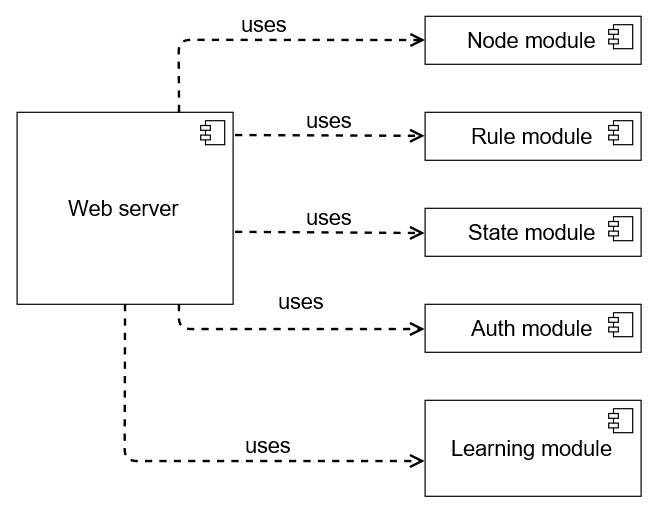
\includegraphics[width=0.6\textwidth]{imagens/componentes_servidor.png}
  \label{fig:componentes_servidor}  
\end{figure}

O diagrama explicita seis componentes no servidor. O servidor \textit{web} essencialmente escuta por requisições contendo mensagens JSON do protocolo Homecloud, descritas na seção \ref{subsec:hc_sintaxe}. Além disso, ele efetua a manutenção das sessões dos agentes do sistema. No entanto, o tratamento das mensagens são feitas chamando funções dos módulos de Nós, Regras, Estado e de Autenticação.

Cada um dos módulos citados lida com as mensagens de seu respectivo tipo, conforme classificação apresentada na seção \ref{subsec:hc_sintaxe}. Esses módulos expõem funções seguindo uma interface definida que podem ser referenciadas pelo servidor \textit{web} para tratar as mensagens recebidas.

Para implementação do servidor, foi utilizada a linguagem Clojure\footnote{Disponível em \url{https://clojure.org/}.}. O Clojure foi utilizado por ser uma linguagem funcional altamente paralelizável, contribuindo para a escalabilidade do servidor. Isso se dá pelo fato de as estruturas da linguagem serem imutáveis por padrão, somado ao de as referências serem \textit{thread-safe}.

O banco de dados utilizado no servidor foi o MongoDB\footnote{Disponível em \url{https://www.mongodb.com/}.}. O MongoDB é um banco de dados NoSQL orientado a documentos. Diferentemente dos banco de dados relacionais, o MongoDB não exige que se faça uma definição da estrutura dos dados armazenados nas tabelas. Em vez disso, ele trabalha com uma estrutura denominada ``documento'', que se assemelha a um objeto JSON. A vantagem dele é a possibilidade de documentos em uma mesma coleção possuírem estruturas distintas. Isso permite, por exemplo, que se construa uma coleção de nós para uma casa englobando tanto atuadores (que possuem uma estrutura de comandos) e sensores (que possuem uma de dados).

A relação entre as coleções do banco de dados estão esquematizadas através do diagrama da Figura \ref{fig:servidor_bd}.

\begin{figure}[h]
	\centering
	\caption{Diagrama de relacionamentos explicitando as coleções utilizadas no banco de dados do servidor.}
  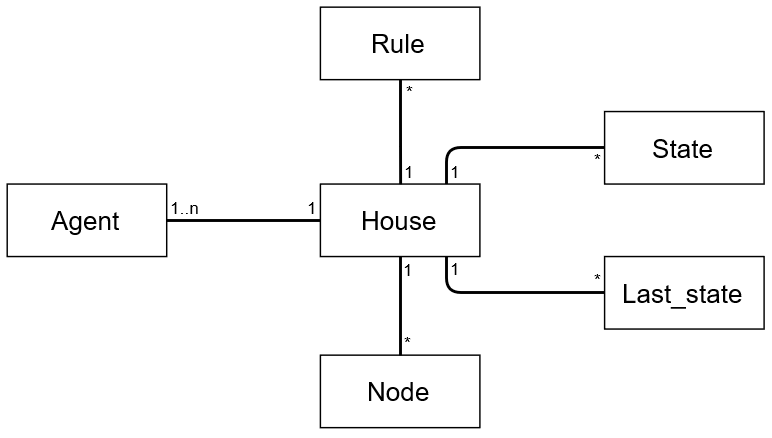
\includegraphics[width=0.7\textwidth]{imagens/servidor_bd.png}
  \label{fig:servidor_bd}  
\end{figure}

Observe que existem seis coleções definidas em uma casa. A coleção \texttt{house} agrupa todos os itens em uma abstração de ``casa'', permitindo que se façam \textit{queries} da natureza ``Obtenha todos os nós da casa a que eu (usuário) estou associado)'', ou ``Obtenha o estado da minha casa''. Todas as relações são do tipo ``um para muitos'', notando-se que a relação entre \texttt{house} e \texttt{agent} possui participação obrigatória de ambas as partes.

O código-fonte do servidor está disponível no repositório GitHub\footnote{Disponível em \url{https://github.com/HomeSkyLtd/server/tree/ws}.}.

\subsection{Implementação de Biblioteca para Aplicativo}
De modo similar ao servidor, a implementação do suporte ao protocolo Homecloud no aplicativo também foi feito de forma modular. Especificamente, foi desenvolvida uma biblioteca que pode ser utilizada como dependência em projetos Android para efetuar a troca de mensagens seguindo o protocolo, conforme ilustra a Figura \ref{fig:arquitetura_lib_app}. A Figura \ref{fig:classes_lib_app} apresenta um diagrama de classes ilustrando a estrutura da biblioteca.

\begin{figure}[h]
	\centering
	\caption{Estrutura modular (em camadas) do desenvolvimento de aplicativo.}
  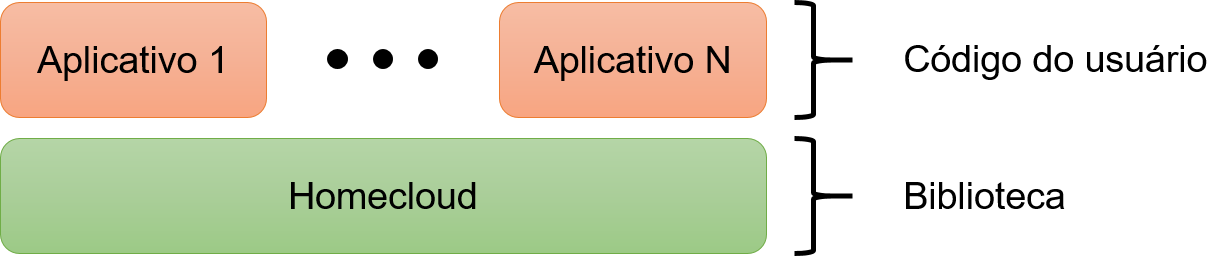
\includegraphics[width=0.7\textwidth]{imagens/arquitetura_lib_app.png}
  \label{fig:arquitetura_lib_app}  
\end{figure}

\begin{figure}[h]
	\centering
	\caption{Diagrama de classes mostrando a estrutura da biblioteca para aplicativos.}
  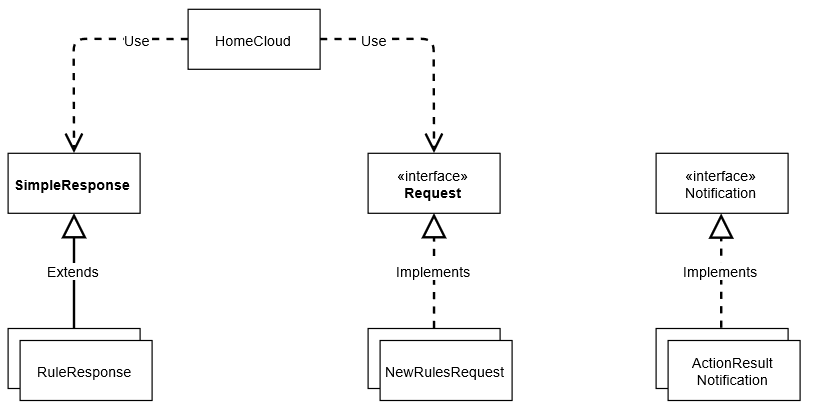
\includegraphics[width=0.7\textwidth]{imagens/classes_lib_app.png}
  \label{fig:classes_lib_app}  
\end{figure}

A interface a ser utilizada pelo aplicativo está contida majoritariamente na classe \texttt{HomeCloud}. Esta classe contém métodos que permitem efetuar todas as requisições do protocolo que envolvam o aplicativo, utilizando, para tanto, classes que implementam a interface \texttt{Request}. Conforme mencionado, cada requisição ao servidor possui uma resposta associada, que é retornada ao aplicativo cliente através da classe \texttt{SimpleResponse} ou de uma de suas filhas.

A biblioteca também lida com notificações recebidas pelo dispositivo, através das classes que implementam a interface \texttt{Notification}. Não existe dependência entre estas classes e a classe \texttt{HomeCloud}, pois foi decidido por deixar sob responsabilidade do usuário a captura dos dados de notificação. Tais classes, então, são acessíveis diretamente pelo usuário, e possuem métodos de \textit{parse} que recebem os dados de uma notificação e retornam um objeto que permita à aplicação interagir de forma conveniente com os dados recebidos.

A implementação da biblioteca foi feita na linguagem Java, e o código-fonte documentado, bem como um aplicativo de demonstração, estão disponíveis no repositório GitHub\footnote{Disponível em \url{https://github.com/HomeSkyLtd/homecloud-app}.}.

\subsection{Implementação de Biblioteca para Controlador}
Seguindo o padrão de desenvolvimento utilizado no projeto, a implementação
do Controlador em si foi desacoplada da implementação da comunicação
com o servidor. Conforme apresentado em \ref{sec:implsens}, a implementação
da rede de sensores local foi realizada em Javascript utilizando o
ambiente Node.js, portanto, a implementação da biblioteca também foi
realizada utilizando-se estas tecnologias.

A biblioteca expõe funções para que o Controlador envie e receba mensagens do servidor seguindo o protocolo Homecloud, realizando de forma transparente ao usuário da biblioteca a autenticação junto ao servidor, a conexão do WebSocket e o enfileiramento das mensagens quando não é possível efetuar o seu envio.

O código-fonte foi hospedado no repositório GitHub\footnote{Disponível em \url{https://github.com/HomeSkyLtd/homecloud-controller}.}. Além disso, a 
biblioteca foi disponibilizada na npm\footnote{Disponível em \url{https://www.npmjs.com/package/homecloud-controller}.}, que além de um gerenciador de pacotes para o Node.js, é um repositório público de bibliotecas.

\subsection{Limitações e Não-escopos} \label{subsec:limit_serv_app}
Os seguintes itens foram considerados fora do escopo deste projeto, no que tange à implementação do protocolo Homecloud, do servidor web e do aplicativo móvel:

\begin{itemize}
	\item Comunicação segura entre dispositivos. A comunicação entre o controlador, o servidor web e o aplicativo móvel deve ser segura, visto que dados confidenciais são trafegados entre as partes. No entanto, a adoção de protocolos subjacentes seguros (como HTTPS/TLS) não foi adotado neste projeto, permanecendo como trabalho futuro;
	\item Dependência de conexão à Internet. A interação do usuário com o sistema por meio do aplicativo móvel é dependente de conexão à Internet, visto que o aplicativo efetua conexão com o servidor web, somente. A remoção desta dependência poderia ser efetuada implementando-se a comunicação do aplicativo com o controlador local, uma vez que o protocolo Homesky, que rege a comunicação entre os dispositivos da rede local, é independente do estado de conexão à Internet.
\end{itemize}


\section{Desenvolvimento do Algoritmo de Aprendizagem}
Nesta seção, detalha-se o processo de desenvolvimento de um algoritmo de aprendizagem para o domínio de controle de iluminação. O algoritmo recebe como entradas um conjunto de dados descrevendo o estado de sensores e atuadores, provenientes do controlador local, e produz como saídas regras de atuação, condicionais aos estados dos sensores.

\subsection{Formato de Entrada dos Dados}\label{subsec:formatoentrada}
No domínio selecionado para este trabalho, o dado de atuação relevante seria o estado da lâmpada a ser controlada. O objetivo do algoritmo, então, é prever o valor deste estado baseado nas leituras de outros sensores existentes na rede doméstica, tais como de luminosidade e presença. A Tabela \ref{tab:entrada_learning} ilustra o formato de entrada dos dados.

\begin{table}[h]
	\centering
	\caption{Formato dos dados de entrada para o algoritmo de aprendizagem.}\smallskip
	\label{tab:entrada_learning}
	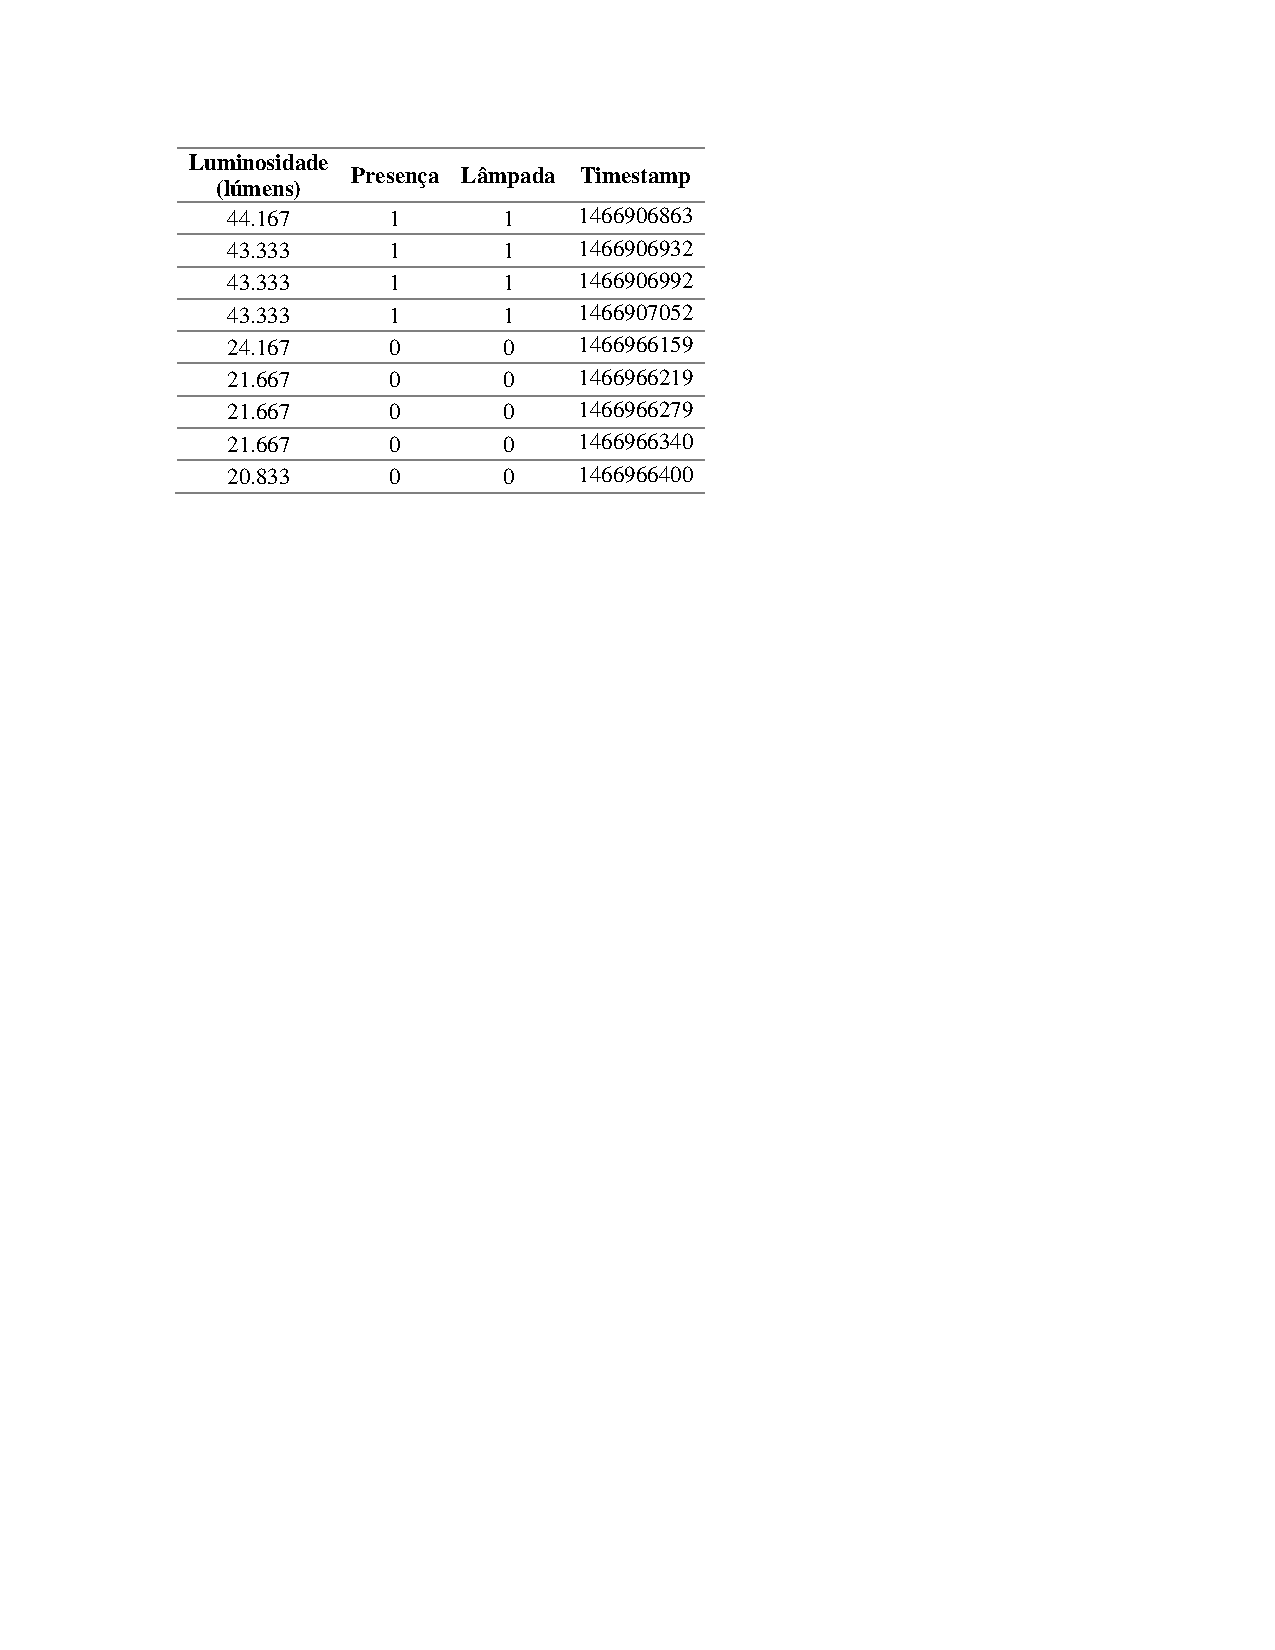
\includegraphics[width=0.5\textwidth]{tabelas/entrada_learning.pdf}
\end{table}

Observe que o problema em questão consiste em receber dados de treino, que representam o comportamento do usuário, e desenvolver um modelo que preveja o estado do atuador de forma fiel aos dados observados. Trata-se, portanto, de um problema de aprendizagem supervisionada, definido em \cite{james2014} como sendo a geração de um modelo que relaciona uma variável-alvo (no caso, o estado da lâmpada) com variáveis preditoras (presença, luminosidade, entre outros). O estado da lâmpada, então, é visto como uma classe associada a cada entrada do conjunto de dados, e o processo de aprendizagem supervisionado que infere esta classe para entradas não vistas anteriormente é denominado Classificação.

\subsection{Algoritmos de Classificação Existentes}\label{subsec:algclass}
Existem diversos algoritmos de classificação documentados na literatura, cada qual adotando uma abordagem distinta para geração de modelos e classificação de dados novos \cite{han2005, james2014}. A seguir serão descritos de forma sucinta três técnicas candidatas a serem utilizadas no processo de derivação de regras para este projeto.

\subsubsection{Indução por Árvore de Decisão}
O modelo de classificação gerado por esta técnica consiste em uma árvore de decisão, em que cada nó interno representa um teste a uma variável preditora, cada aresta representa uma saída do teste, e cada nó terminal (folha) indica a classe resultante. A Figura \ref{fig:exemplo_arvore} mostra o exemplo de uma árvore de decisão obtida por esta técnica. 

Neste exemplo, o conjunto de dados refere-se a consumidores de uma loja de eletrônicos, e as classes mostradas nos nós-folha indicam se um consumidor adquire ou não certo produto. No caso, uma das regras geradas pelo modelo diz que se o consumidor é jovem e estudante, então ele adquire o produto.

\begin{figure}[h]
	\centering
	\caption{Exemplo de modelo gerado pela técnica de Indução por Árvore de Decisão}
  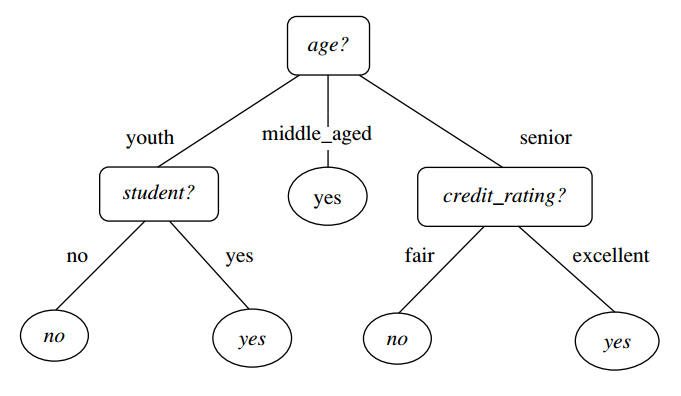
\includegraphics[width=0.8\textwidth]{imagens/exemplo_arvore.png}
  \label{fig:exemplo_arvore}  
  
  Fonte: \cite{han2005}
\end{figure}

Existem diversas implementações desta técnica de classificação, tais como ID3, C4.5 e CART, que adotam uma estratégia \textit{greedy} e \textit{top-down} de construção da árvore. Cada uma dessas implementações efetua o particionamento dos dados de forma particular, efetuando seleção de variáveis por critérios tais como ganho de informação, razão de ganho ou índice Gini. As descrições dessas técnicas fogem do escopo deste trabalho, e podem ser encontradas em \cite{han2005}.

\subsubsection{Redes Neurais}
A técnica de aprendizagem por redes neurais foi inspirada pelos ramos da psicologia e neurobiologia, que buscaram modelar computacionalmente o comportamento de neurônios. Uma rede neural é composta por diversas unidades interconectadas arranjadas em camadas, conforme ilustra a Figura \ref{fig:elem_rede_neural}. 

Os dados de entrada do classificador são passados para as unidades da camada de entrada. Esses dados, então, são combinados linearmente através de pesos determinados nas interconexões e passados às unidades das camadas intermediárias, denominadas \textit{hidden layers}. As saídas da última camada intermediária são passadas às unidades da camada de saída, que define a classe resultante.

\begin{figure}[h]
	\centering
	\caption{Elementos de uma rede neural}
  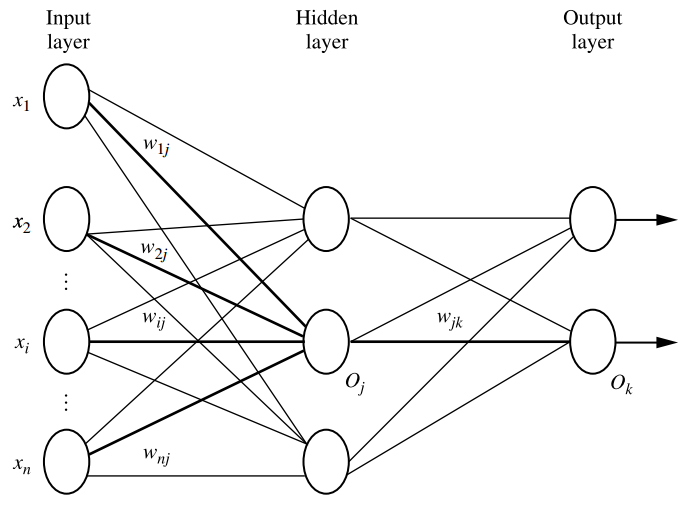
\includegraphics[width=0.8\textwidth]{imagens/elem_rede_neural.png}
  \label{fig:elem_rede_neural}  
  
  Fonte: \cite{han2005}
\end{figure}

O processo de aprendizagem das redes neurais é computacionalmente caro e complexo, envolvendo um processo denominado \textit{backpropagation}. Este é um processo iterativo que consiste em alimentar os dados de treino na rede neural, obter a saída com o modelo corrente, e reajustar os pesos do modelo em ordem reversa, partindo das unidades da camada de saída.

No entanto, as redes neurais possuem a vantagem de possuírem alta tolerância a dados ruidosos, além de não requerer conhecimento da relação entre as classes a serem previstas e as variáveis preditoras \cite{han2005}.

\subsubsection{\textit{Support Vector Machines} (SVM)}
O SVM é uma técnica de classificação que se baseia na definição de um hiperplano ótimo para efetuar a segregação dos dados pertencentes às diferentes classes. No caso, o hiperplano ótimo seria o que provê maior margem entre os dados, conforme ilustra a Figura \ref{fig:svm_max_margin}. Neste exemplo, o conjunto de dados é bidimensional, e o hiperplano de separação é uma reta. Observe que das diversas retas possíveis mostradas à esquerda, seleciona-se a que resulta em maior margem, mostrada à direita.

\begin{figure}[h]
	\centering
	\caption{Retas candidatas para efetuar a segregação dos dados (esq.), e a reta ótima selecionada, que provê a maior margem no conjunto de dados}
  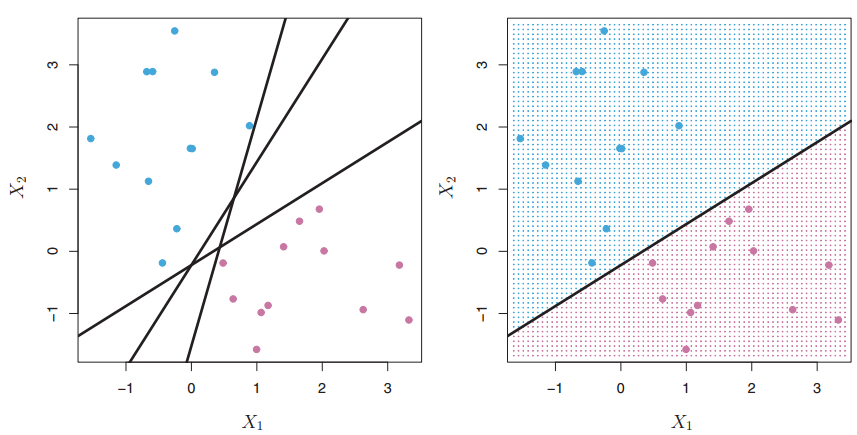
\includegraphics[width=0.8\textwidth]{imagens/svm_max_margin.png}
  \label{fig:svm_max_margin}  
  
  Fonte: \cite{james2014}
\end{figure}

A técnica de SVM se baseia nesta ideia de definir um plano de separação ótimo, mas efetua a adição de mais dimensões aos dados originais para lidar com situações de margens não-lineares. Este aumento na dimensionalidade dos dados é feito com base na utilização de \textit{kernels}. A descrição matemática deste processo está fora do escopo deste trabalho, e pode ser encontrado em \cite{james2014}.

\subsection{Considerações sobre a Escolha do Algoritmo}
A seção \ref{subsec:algclass} apresentou três algoritmos de classificação passíveis de serem aplicados no projeto. Conforme mencionado, cada algoritmo possui uma abordagem distinta na construção do modelo e na avaliação de entradas novas para efetuar a classificação, possuindo vantagens e desvantagens particulares. Esta seção lista as considerações adotadas para a seleção do algoritmo a ser utilizado na geração de regras.

O fator principal utilizado para selecionar o algoritmo de aprendizagem é a interpretabilidade do modelo gerado. Dentre as razões para a priorização deste fator, destaca-se a necessidade de o usuário ter capacidade de analisar as regras propostas pelo algoritmo, de modo a dar-lhe a escolha de aceitá-la ou recusá-la. Essa possibilidade é extremamente importante, levando-se em conta que os sensores utilizados em ambiente doméstico podem possuir imprecisões que resultem na geração de regras estatisticamente precisas, mas ainda assim indesejadas pelo usuário.

Nesse contexto, \cite{james2014} menciona haver um \textit{tradeoff} entre a flexibilidade e a interpretabilidade dos métodos de aprendizagem, como mostra a Figura \ref{fig:interpretabilidade_algoritmos}. Métodos flexíveis possuem alta capacidade de gerar modelos que se adaptem a dados de natureza complexa, mas tais modelos acabam sendo de difícil interpretação pelo usuário. 

\begin{figure}[h]
	\centering
	\caption{\textit{Tradeoff} entre flexibilidade e interpretabilidade de métodos de aprendizagem}
  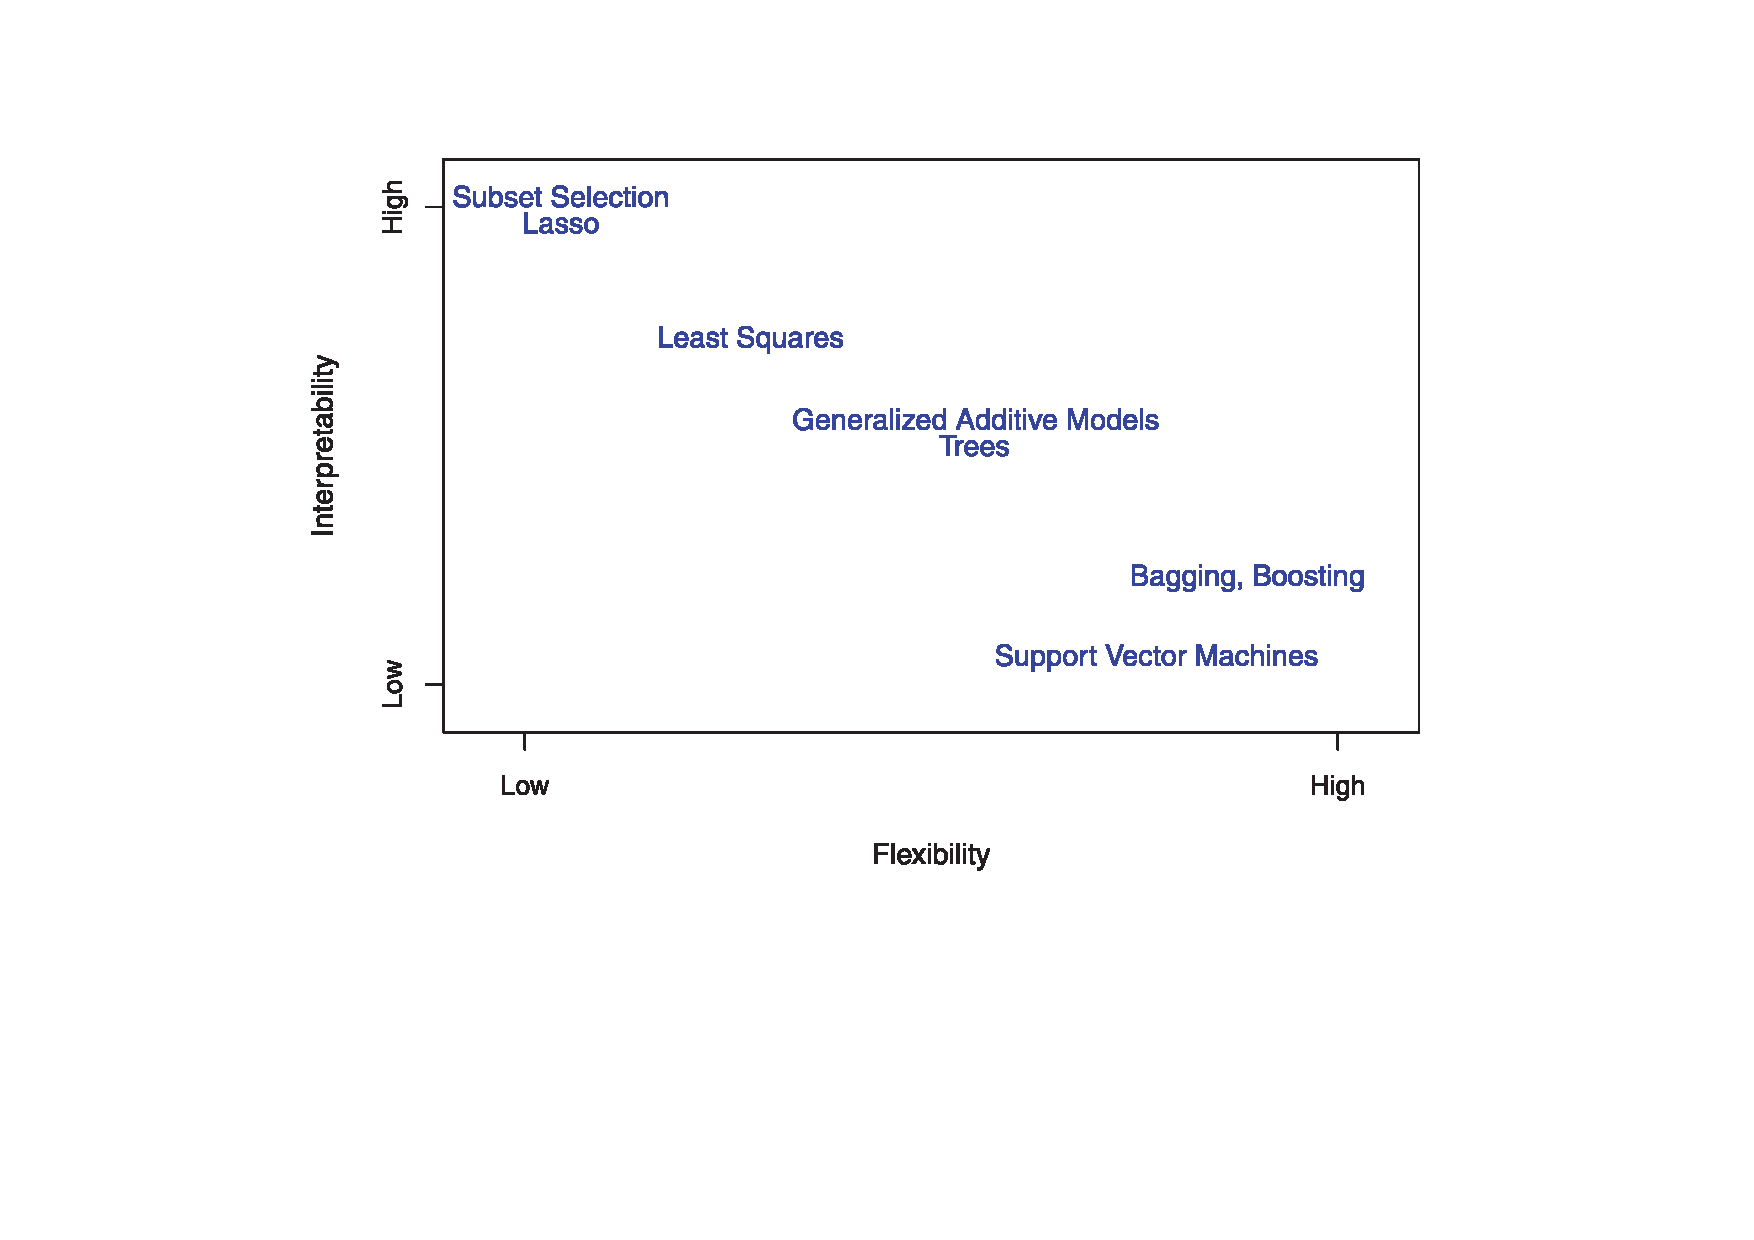
\includegraphics[width=0.8\textwidth]{imagens/interpretabilidade_algoritmos.pdf}
  \label{fig:interpretabilidade_algoritmos}  
  
  Fonte: \cite{james2014}
\end{figure}

Note que, dentre as técnicas apresentadas, redes neurais e SVM possuem alta flexibilidade, permitindo gerar modelos para dados com variáveis cuja relação é desconhecida, a princípio (no caso das redes neurais), e para dados com fronteira de decisão não-linear (no caso do SVM). Entretanto, os modelos gerados por estas técnicas são pouco interpretáveis: redes neurais expõem um conjunto de pesos que processam os dados, de acordo com a topologia selecionada, e o SVM gera um hiperplano de separação.

No extremo oposto encontra-se a técnica de classificação por árvores de decisão. Este método é mais restritivo em termos de flexibilidade, mas gera modelos facilmente interpretáveis. De posse de um modelo como o da Figura \ref{fig:exemplo_arvore}, por exemplo, é intuitivo obter os fatores que influenciam na classificação das entradas.

Pelas razões mencionadas anteriormente, o algoritmo de classificação por árvore de decisão foi adotado para derivar regras de atuação. A seguir serão descritos os experimentos feitos com  dados de iluminação, englobando o preprocessamento dos dados e a aplicação do algoritmo de classificação propriamente dito.

\subsection{Coleta de Dados}
Conforme mencionado, o domínio de aplicação abordado para concepção de um algoritmo de aprendizagem de regras é o de controle de iluminação. Para iniciar os testes, é necessário ter em mãos um \textit{dataset} em formato similar ao descrito na seção \ref{subsec:formatoentrada}. Para obter tais dados de treino, os membros do grupo adquiriram sensores de presença PIR e de iluminação, associando-os a um Raspberry Pi, a fim de coletar dados nas respectivas residências. A Figura \ref{fig:montagem_coleta} mostra as montagens utilizadas para efetuar as coletas nas residências.

\begin{figure}[h]
	\centering
	\caption{Montagens experimentais para coleta de dados de iluminação}
	\smallskip
  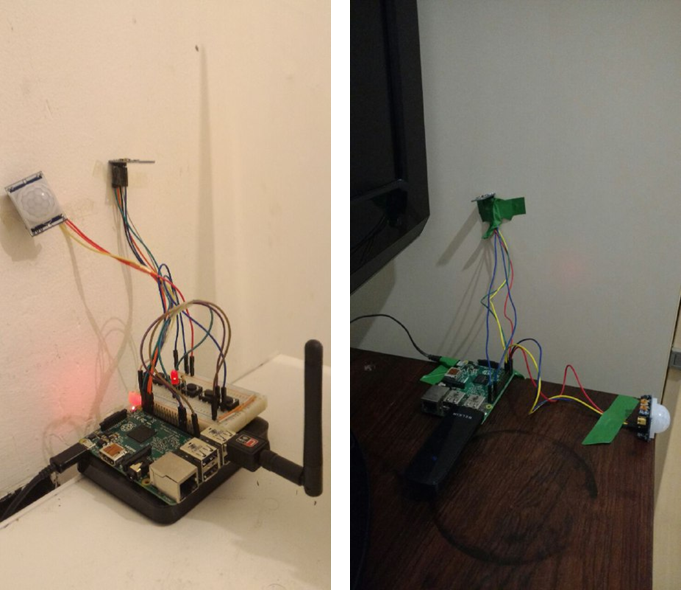
\includegraphics[width=\textwidth]{imagens/montagem_coleta.png}
  \label{fig:montagem_coleta}  
\end{figure}

Neste processo, os dados foram amostrados a cada minuto. Na primeira e terceira montagens (à esquerda e à direita, respectivamente), foi utilizado um botão para sinalizar o momento em que o interruptor foi acionado, devido à inviabilidade de conectar o interruptor existente no processo de coleta. Os dados coletados por estas montagens serão referidos por \textit{dataset} 1 e \textit{dataset} 3 (primeira e terceira montagens, respectivamente). Na segunda montagem (imagem central), o estado do interruptor foi inferido posteriormente, de acordo com o horário do dia e da iluminação ambiente. Os dados coletados por esta montagem serão denominados \textit{dataset} 2. O \textit{timestamp}, mostrado na Tabela \ref{tab:entrada_learning}, foi registrado para cada amostra coletada, e consiste na representação POSIX do instante de coleta do dado.

\subsection{Experimentos para Derivação de Regras}
Como mencionado, o grupo pretende usar um algoritmo de classificação baseado em árvore de decisão para gerar as regras de atuação. Levando em conta a rotina associada aos dados de treino coletados, o grupo espera, idealmente, que as seguintes regras sejam derivadas:
\begin{itemize}
	\item Acenda a luz quando há alguém no ambiente, e a iluminação no local é baixa;
	\item Apague a luz quando não há ninguém no ambiente
\end{itemize}

Para a geração das árvores de decisão, o grupo usou a ferramenta Rattle\footnote{Disponível em \url{http://rattle.togaware.com/}.}, que utiliza um algoritmo recursivo \textit{top-down} \cite{williams2011} implementado na biblioteca \texttt{rpart}\footnote{Documentação disponível em \url{https://cran.r-project.org/web/packages/rpart/index.html}}. O objetivo, nesta seção, é estudar modos de preprocessamento dos dados utilizados pelo algoritmo, e analisar a qualidade das regras criadas. Todo o processamento efetuado sobre os dados foi feito utilizando a linguagem R\footnote{Disponível em \url{https://www.r-project.org/}}.

\subsubsection{Utilização de dados \textit{raw}}
A primeira tentativa de geração de regras foi feita alimentando o algoritmo de geração do modelo sem efetuar nenhum tipo de preprocessamento dos dados. A quantidade de pontos utilizados para cada \textit{dataset} está listada a seguir.

\begin{itemize_compact}
	\item \textit{Dataset} 1
	\begin{itemize_compact}
		\item 3818 pontos com luz ligada
		\item 15454 pontos com luz desligada
	\end{itemize_compact}
		\item \textit{Dataset} 2
	\begin{itemize_compact}
		\item 2398 pontos com luz ligada
		\item 51880 pontos com luz desligada
	\end{itemize_compact}
		\item \textit{Dataset} 3
	\begin{itemize_compact}
		\item 2640 pontos com luz ligada
		\item 16292 pontos com luz desligada
	\end{itemize_compact}
\end{itemize_compact}

Os resultados obtidos estão apresentados na Figura \ref{fig:teste_1}, para cada \textit{dataset} utilizado. Para auxiliar na interpretabilidade dos dados, tenha em mente que valores de luminância na ordem de 40 lx correspondem a um ambiente noturno, com uma lâmpada acesa.

\begin{figure}[hp]
	\centering
	\caption{Árvores de decisão geradas sem nenhum preprocessamento de dados.}
  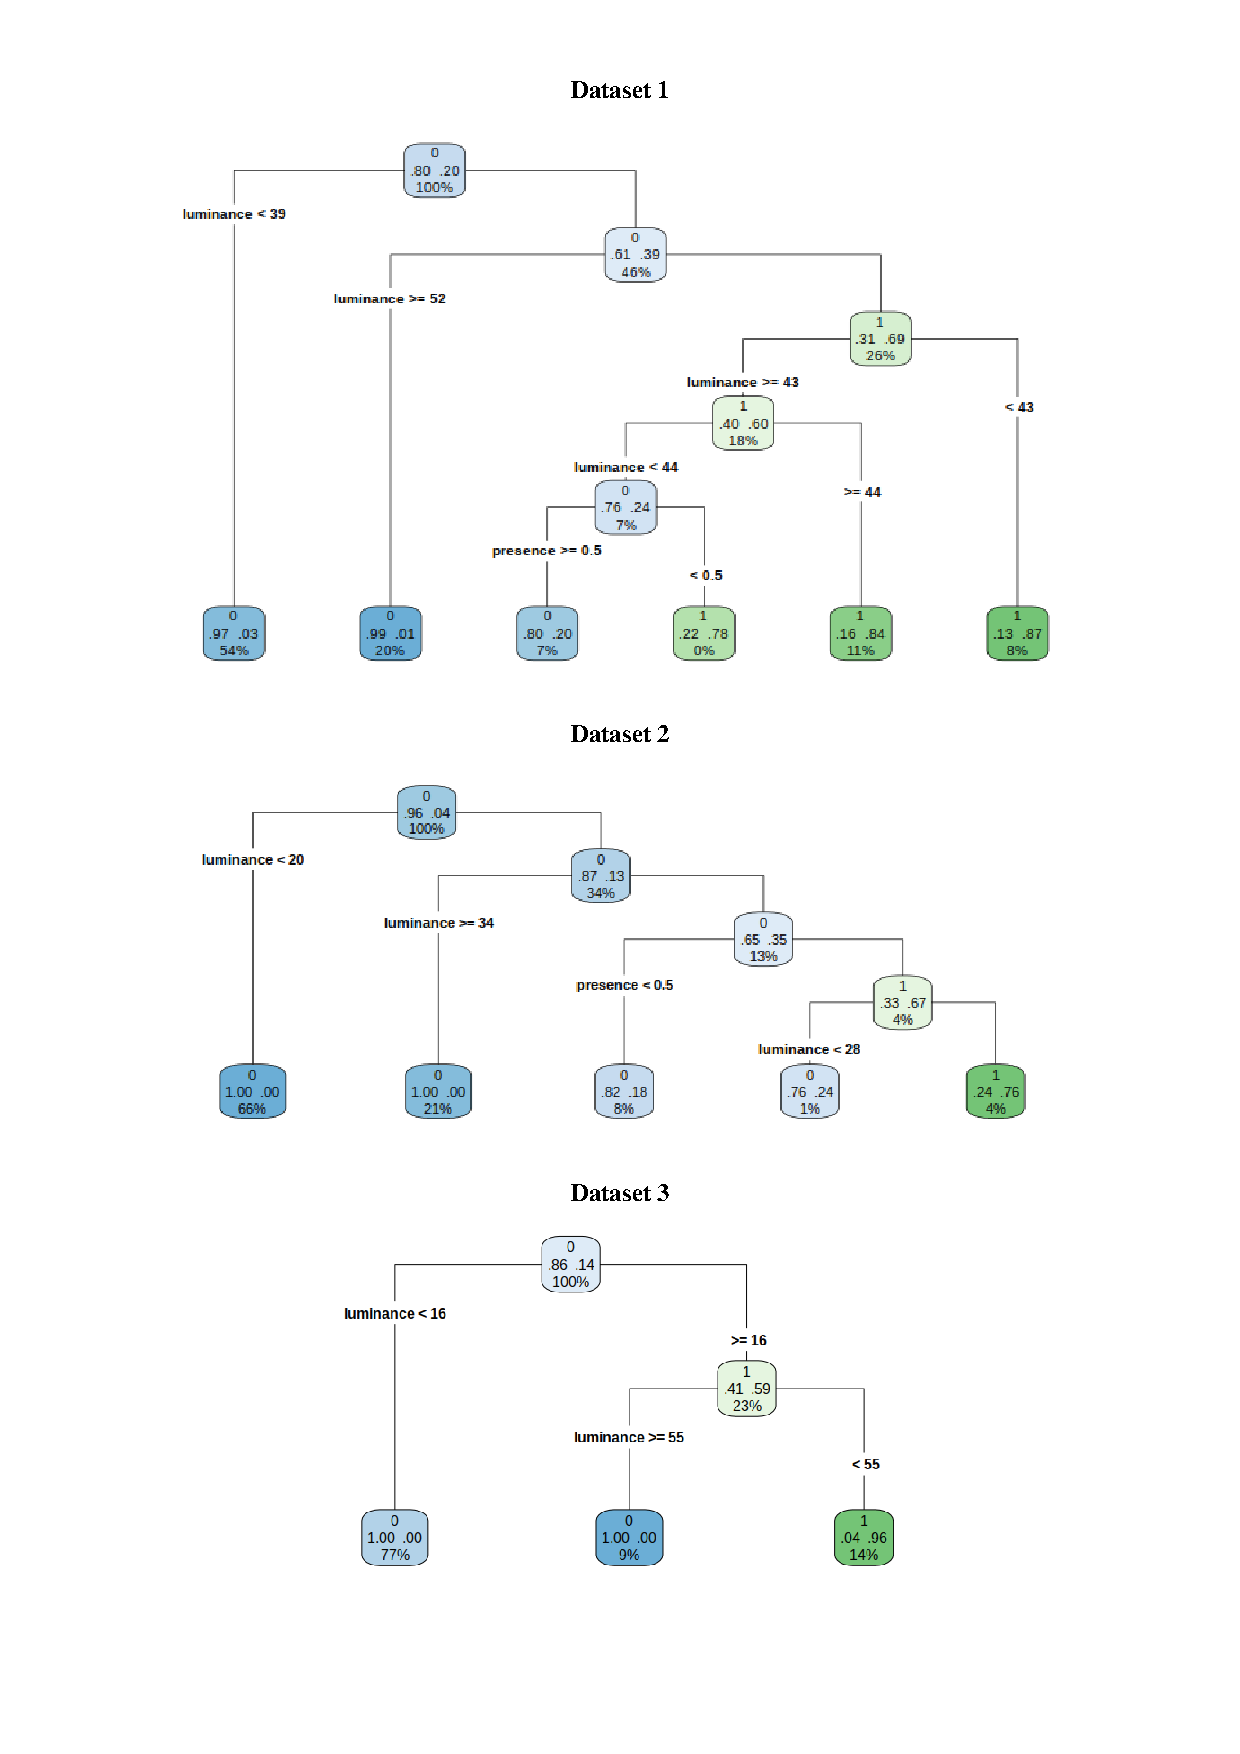
\includegraphics[width=0.8\textwidth]{imagens/teste_learning/1.pdf}
  \label{fig:teste_1}  
\end{figure}

Para fins de criação de regras, o interesse maior está em identificar o estado em que ocorreu uma mudança no estado da lâmpada. Para tanto, torna-se necessário efetuar um preprocessamento dos dados para evidenciar essas mudanças no \textit{dataset}.

\clearpage

\subsubsection{Adição de um campo de Ação}
Nesta tentativa, foi efetuado um passo de preprocessamento adicionando uma coluna indicando a ação tomada no instante. Por exemplo, se em um dado instante a lâmpada está apagada, mas no seguinte ela está acesa, então o campo ``Ação'' assume valor ``1'', indicando que a lâmpada foi acesa. Analogamente, se a lâmpada está acesa em um dado instante e no seguinte ela está apagada, então o campo ``Ação'' assume valor ``-1'', indicando que ela foi apagada. Caso o estado da lâmpada seja o mesmo em dois instantes de tempo consecutivos, o campo ``Ação'' assume valor ``0'', indicando ausência de ação.

Efetuando este tratamento, a quantidade de pontos em cada \textit{dataset} se encontra distribuída conforme listado a seguir.

\begin{itemize_compact}
	\item \textit{Dataset} 1
	\begin{itemize_compact}
		\item 19228 pontos sem ação
		\item 22 pontos ligando a luz
		\item 22 pontos apagando a luz
	\end{itemize_compact}
		\item \textit{Dataset} 2
	\begin{itemize_compact}
		\item 54094 pontos sem ação
		\item 92 pontos ligando a luz
		\item 92 pontos apagando a luz
	\end{itemize_compact}
		\item \textit{Dataset} 3
	\begin{itemize_compact}
		\item 18871 pontos sem ação
		\item 31 pontos ligando a luz
		\item 30 pontos apagando a luz
	\end{itemize_compact}
\end{itemize_compact}

A Figura \ref{fig:teste_2} ilustra os resultados obtidos após efetuar este preprocessamento.

\begin{figure}[hp]
	\centering
	\caption{Árvores de decisão geradas após processamento dos dados, adicionando-se campo de ação.}
  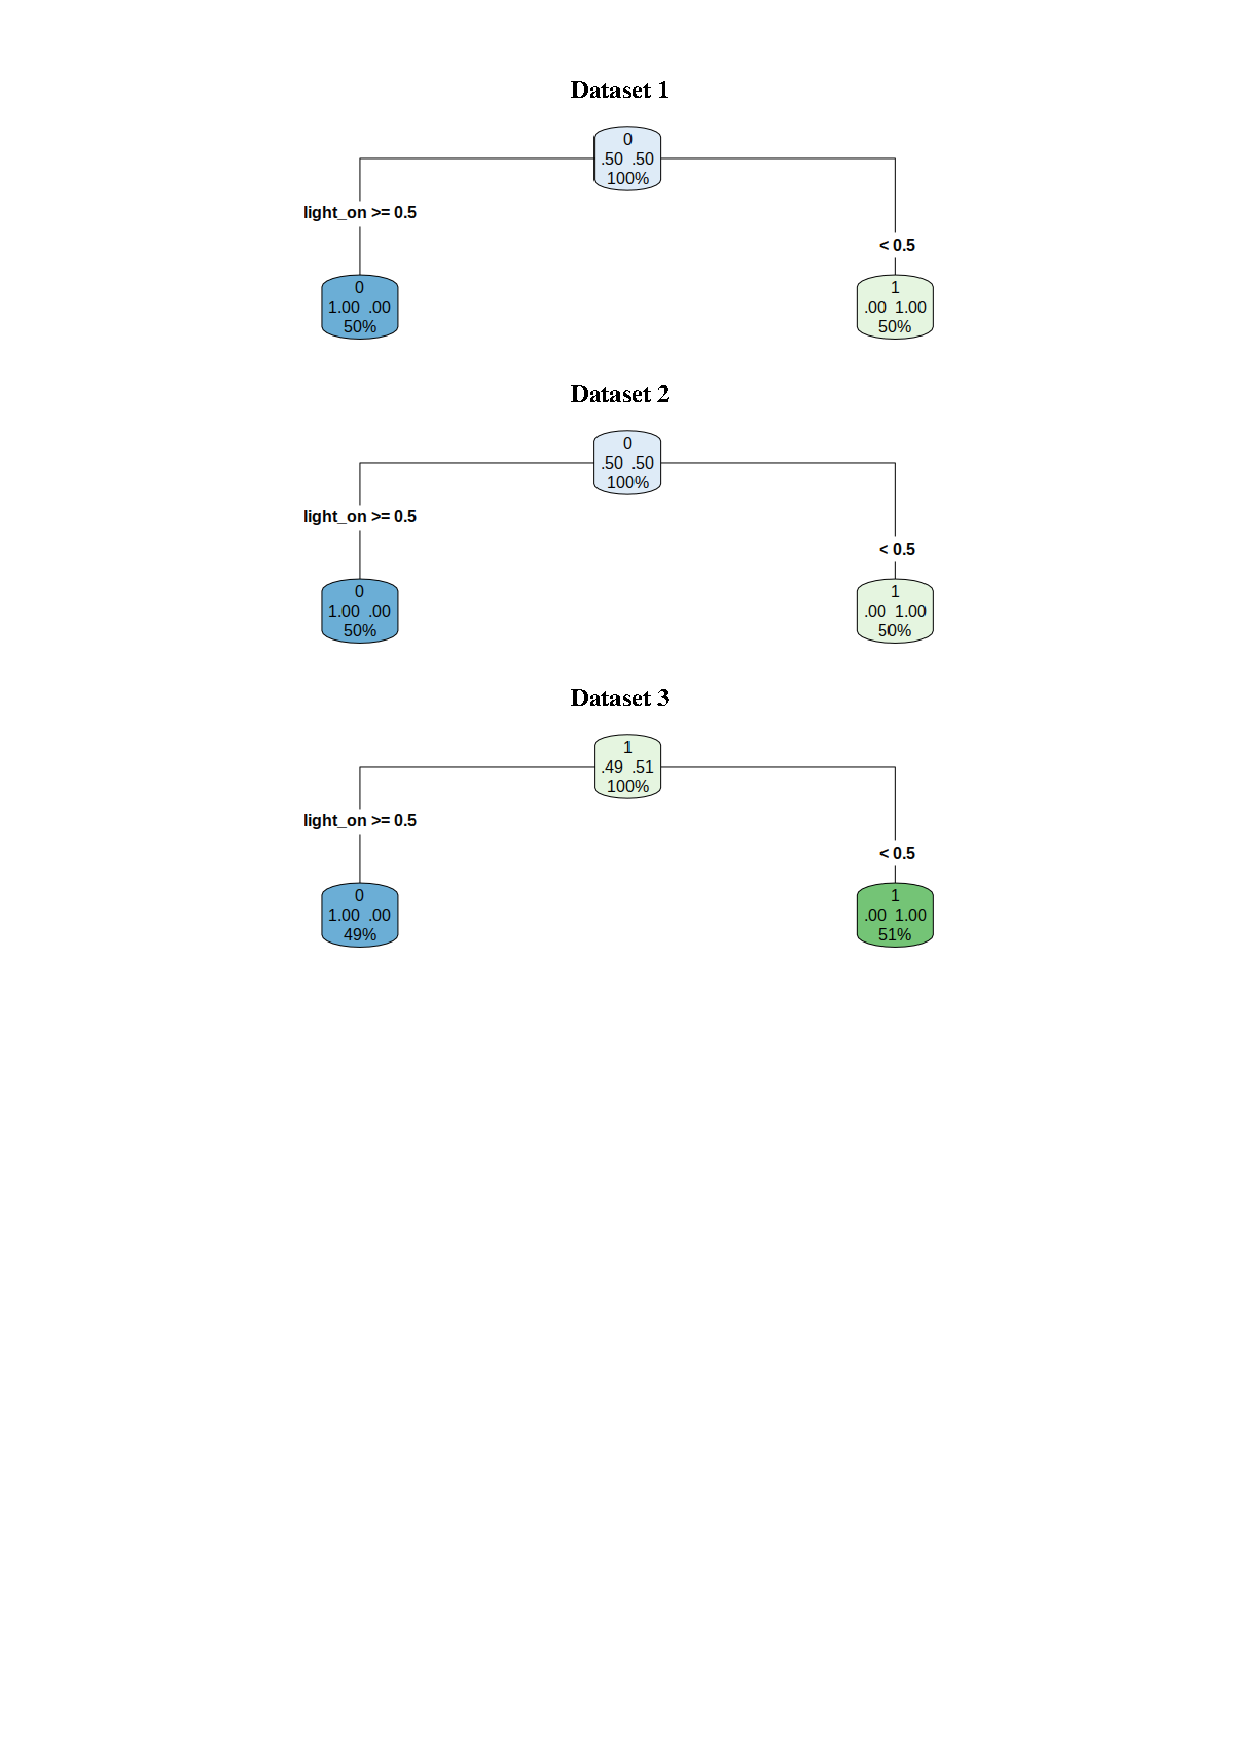
\includegraphics[width=0.8\textwidth]{imagens/teste_learning/2.pdf}
  \label{fig:teste_2}  
\end{figure}

\clearpage

\subsubsection{Eliminação dos pontos sem ação} \label{subsubsec:elim_pts_sem_acao}
Esta tentativa buscou explorar a eficácia do algoritmo caso pontos sem ação (Ação=0) fossem eliminados. A Figura \ref{fig:teste_3} mostra as árvores de decisão geradas nesta tentativa.

\begin{figure}[hp]
	\caption{Árvores de decisão geradas mantendo somente pontos com ação tomada.}
	\smallskip
	\begin{subfigure}{\textwidth}
		\centering
  	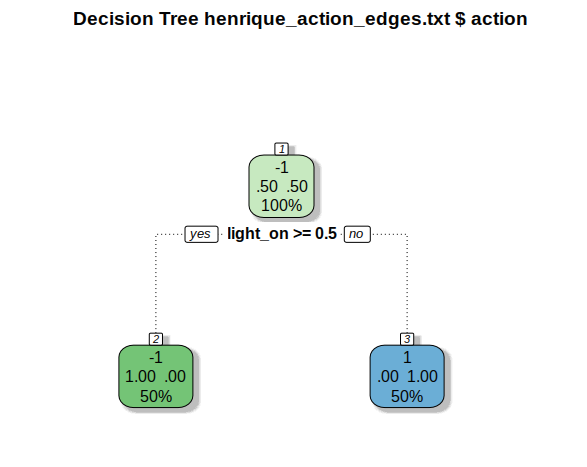
\includegraphics[width=0.8\textwidth]{imagens/teste_learning/3_h.png}
  \end{subfigure}
  	\begin{subfigure}{\textwidth}
		\centering
  	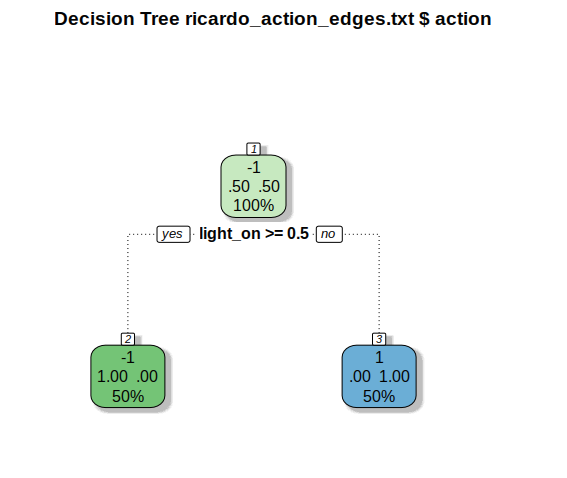
\includegraphics[width=0.8\textwidth]{imagens/teste_learning/3_r.png}
  \end{subfigure}
  \label{fig:teste_3}  
\end{figure}

Observe que as regras geradas ditam que a luz seja apagada, caso ela esteja acesa, e vice-versa. De fato, do universo de pontos coletados neste item, é óbvio que a luz sempre é apagada quando ela está acesa, e ela sempre é acesa quando está apagada. Ocorre que a eliminação dos dados de Ação=0, apesar de resolver o problema de desbalanceamento, introduziu uma perda de informação significativa. Ocorre que, em diversos momentos em que a luz está acesa, ela não é apagada. A manutenção de tais pontos, pois, se mostra imprescindível para a geração de regras coerentes.

\subsubsection{Balanceamento do \textit{dataset}}
Conforme mencionado, o \textit{dataset} em questão é extremamente desbalanceado, com uma quantidade de entradas com classe Ação=0 ordens de grandeza maior que entradas das demais classes. Conforme mencionado em \cite{han2005}, dentre as técnicas utilizadas para se lidar com problemas de classificação desbalanceados estão o \textit{undersampling} da classe majoritária e o \textit{oversampling} da classe minoritária. Neste teste, a primeira técnica será adotada para reduzir a quantidade de entradas da classe Ação=0.

O \textit{undersample} foi efetuado selecionando-se uma quantidade de pontos da classe majoritária de forma aleatória. A Figura \ref{fig:teste_4} mostra as árvores de decisão geradas nesta tentativa.

\begin{figure}[hp]
	\caption{Árvores de decisão geradas efetuando \textit{undersample} da classe majoritária.}
	\smallskip
	\begin{subfigure}{\textwidth}
		\centering
  	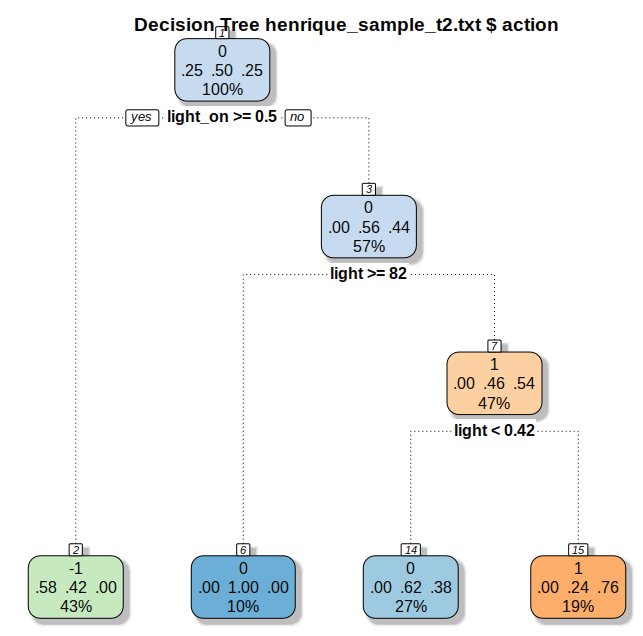
\includegraphics[width=0.7\textwidth]{imagens/teste_learning/4_h.png}
  \end{subfigure}
  	\begin{subfigure}{\textwidth}
		\centering
  	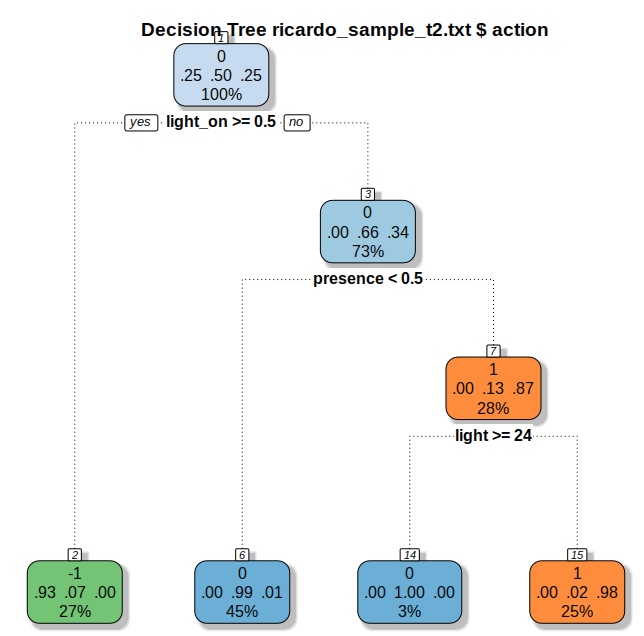
\includegraphics[width=0.7\textwidth]{imagens/teste_learning/4_r.png}
  \end{subfigure}
  \label{fig:teste_4}  
\end{figure}

No \textit{dataset} 1, as regras produzidas foram:
\begin{itemize}
	\item Apague a luz quando ela estiver acesa ($light\_on >= 0.5$)
	\item Acenda a luz quando ela estiver apagada e a iluminação ambiente estiver entre 0.42 e 82
	\item Não faça nada caso contrário
\end{itemize}
No caso do segundo \textit{dataset}, as regras produzidas foram:
\begin{itemize}
	\item Apague a luz quando ela estiver acesa ($light\_on >= 0.5$)
	\item Acenda a luz quando ela estiver apagada, alguém estiver no quarto e a iluminação ambiente for menor que 24
	\item Não faça nada, caso contrário
\end{itemize}

Como foi efetuado uma amostragem aleatória em todos os pontos de não ação, reproduzimos esse teste diversas vezes, e as árvores resultantes são as que ocorriam com mais frequência nos testes. Em ambas as árvores, observa-se que ele derivou a regra para apagar a luz sempre que ela esteja acesa, e apenas no segundo \textit{dataset} utilizou a presença no caso de acender a luz.

Analisando o \textit{dataset}, observa-se que acontece de o usuário acender a luz antes da presença ser detectada e também de apagá-la ainda sob alcance do sensor de presença. Ou seja, o usuário deixa o ambiente quando apaga a luz e o frequenta quando a acende, e essa informação não é representada tomando unicamente a leitura instantânea do sensor de presença.

\subsubsection{Consideração de médias temporais dos dados}
Com o intuito de capturar o estado do ambiente associado à tomada de uma ação, testou-se a utilização de uma média temporal de $n$ pontos para a presença, em vez de utilizar uma única medida instantânea. Deste modo, para um dado instante, o valor da presença é a média dos $n$ valores subsequentes, arranjados de forma temporal. Efetuar este tipo de processamento faz com que os \textit{datasets} reflitam o estado do ambiente após a tomada da ação, contribuindo para a geração de regras mais precisas. No entanto, há a necessidade de se conhecer a natureza dos dados coletados para que este tipo de processamento faça sentido, tornando este tratamento específico para a aplicação descrita de controle de iluminação.

A Figura \ref{fig:teste_5_1} mostra árvores de decisão geradas para o \textit{dataset} 1, ao passo que a Figura \ref{fig:teste_5_2} mostra as geradas para o \textit{dataset} 2. Nestes modelos, foi utilizado $n=10$. Devido à natureza aleatória do \textit{undersampling}, as duas árvores apresentadas em cada figura foram geradas frequentemente.

\begin{figure}[hp]
	\caption{Árvores de decisão geradas para o \textit{dataset} 1 tomando a média temporal da presença, com $n=10$.}
	\smallskip
	\begin{subfigure}{\textwidth}
		\centering
  	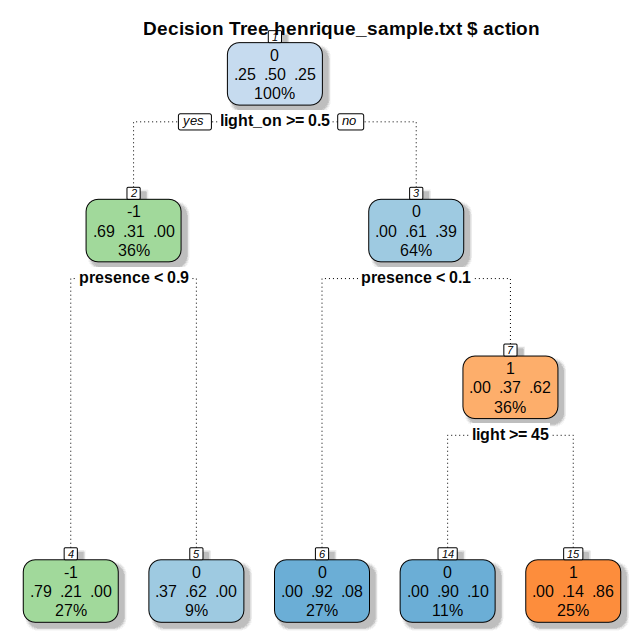
\includegraphics[width=0.7\textwidth]{imagens/teste_learning/5_h_1.png}
  \end{subfigure}
  	\begin{subfigure}{\textwidth}
		\centering
  	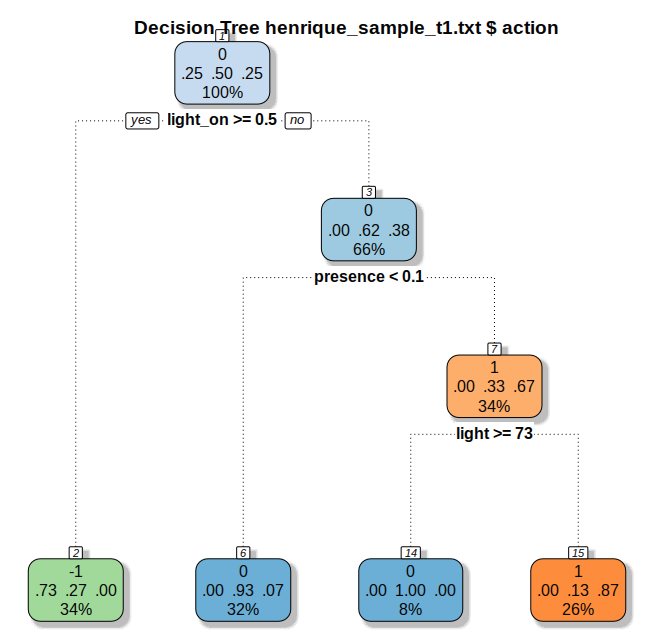
\includegraphics[width=0.7\textwidth]{imagens/teste_learning/5_h_2.png}
  \end{subfigure}
  \label{fig:teste_5_1}  
\end{figure}

\begin{figure}[hp]
	\caption{Árvores de decisão geradas para o \textit{dataset} 2 tomando a média temporal da presença, com $n=10$.}
	\smallskip
	\begin{subfigure}{\textwidth}
		\centering
  	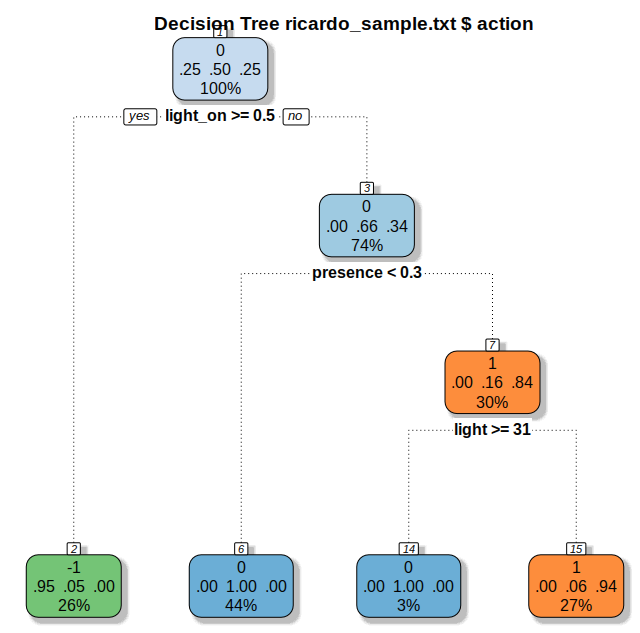
\includegraphics[width=0.7\textwidth]{imagens/teste_learning/5_r_1.png}
  \end{subfigure}
  	\begin{subfigure}{\textwidth}
		\centering
  	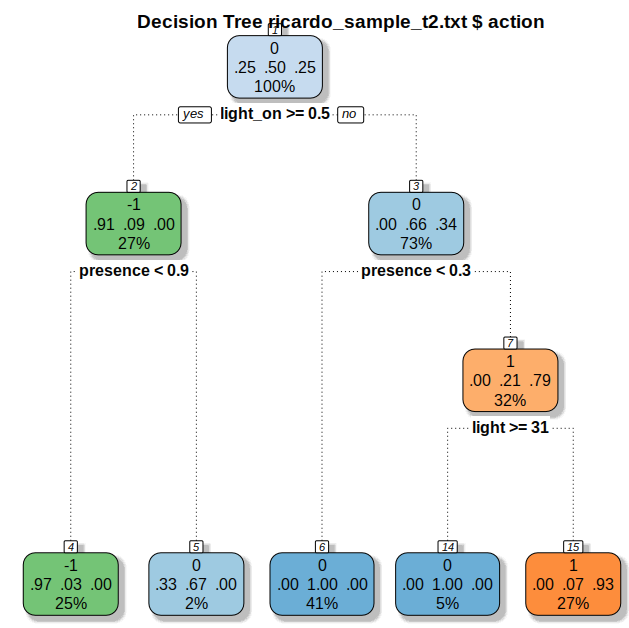
\includegraphics[width=0.7\textwidth]{imagens/teste_learning/5_r_2.png}
  \end{subfigure}
  \label{fig:teste_5_2}  
\end{figure}

Observe que os resultados obtidos são similares para os dois \textit{datasets}. Analisando a primeira árvore da Figura \ref{fig:teste_5_1}, observa-se que as regras geradas foram:
\begin{itemize}
	\item Apague a luz quando ela estiver acesa e não houver ninguém no ambiente;
	\item Acenda a luz quando ela estiver apagada, houver presença no ambiente e o nível de luminosidade for menor que 45;
	\item Não faça nada caso contrário.
\end{itemize}
No caso da segunda árvore da Figura \ref{fig:teste_5_1}, tem-se as regras:
\begin{itemize}
	\item Apague a luz quando ela estiver acesa;
	\item Acenda a luz quando ela estiver apagada, houver presença no ambiente e o nível de luminosidade for menor que 73;
	\item Não faça nada caso contrário.
\end{itemize}

Observe que a primeira árvore obtida gerou regras ótimas, levando em conta os \textit{datasets} utilizados. A segunda, no entanto, ainda sugeria regras que simplesmente apagavam a luz quando ela estivesse acesa. Este problema é similar ao obtido no teste \ref{subsubsec:elim_pts_sem_acao}, e provavelmente se deve ao fato de não terem sido escolhidos pontos suficientes da classe Ação=0 no processo de \textit{undersampling}.

\subsubsection{\textit{Undersampling} com clusterização}
Uma maneira de melhorar o processo de \textit{undersampling}, de modo que os dados coletados representem mais fielmente o \textit{dataset} original, seria aplicar técnicas de clusterização à classe majoritária. Desse modo, o procedimento de amostragem consistiria em coletar alguns pontos de cada cluster identificado.

O algoritmo de clusterização utilizado nesta etapa foi o CLARA (\textit{Clustering LARge Applications}), que é classificado como um algoritmo de clusterização por particionamento \cite{han2005}. O CLARA é resultado de uma série de incrementos efetuados sobre outros algoritmos de particionamento, partindo do mais simples: o \textit{k-means}.

O \textit{k-means} é um algoritmo de clusterização iterativo que utiliza a noção de centroides como pontos representativos de um cluster. Um centroide pode ser visto como o centro geométrico de um \textit{dataset}. Os clusters são definidos da seguinte forma. Seja $C=\{c_1,c_2,...,c_k\}$ o conjunto de pontos representativos (centroides), onde $k$ é o número de clusters, e $dist(x,y)$ uma função de cálculo de distância entre dois pontos (por exemplo, distância euclidiana). Para cada ponto $p$ do \textit{dataset}, $p$ é alocado ao cluster correspondente ao centroide $c_i$ que minimize $dist(p,c_i)$. 

Inicialmente, os $k$ centroides são escolhidos de forma aleatória do \textit{dataset}. Então, o algoritmo efetua dois passos de forma iterativa:
\begin{enumerate}
	\item Aloque cada ponto $p$ ao cluster correspondente, seguindo o procedimento descrito anteriormente;
	\item Recalcule os centroides, atualizando $C$.
\end{enumerate}

O procedimento listado é repetido até que não haja nenhuma alteração nos centroides calculados. A Figura \ref{fig:kmeans} mostra um exemplo de aplicação do algoritmo, em que centroides são representados pelo símbolo $+$. 

\begin{figure}[h]
	\centering
	\caption{Exemplo de execução do algoritmo \textit{k-means}}
  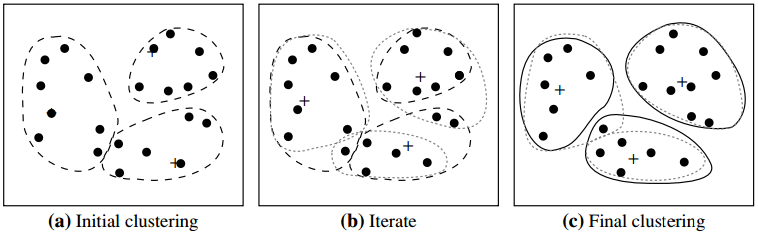
\includegraphics[width=0.8\textwidth]{imagens/kmeans.png}
  \label{fig:kmeans}  
  
  Fonte: \cite{han2005}
\end{figure}

Note que, por definição, os centroides podem não ser coincidentes com um ponto do \textit{dataset}. Isso torna o algoritmo suscetível a valores atípicos (\textit{outliers}), pois a incorporação de tais valores acabaria deslocando os centroides em direção a eles.

Assim, foi proposto um algoritmo que utiliza o conceito de medoide como pontos representativos de um cluster. De modo intuitivo, o medoide $m$ de um \textit{dataset} é um ponto ``central'' pertencente ao \textit{dataset} original. Formalmente, se $P$ é o conjunto de pontos do \textit{dataset}, $m$ é escolhido de tal forma a minimizar $\sum_{p \in P}{dist(m,p)}$, para todo $m \in P$.

A utilização de medoides como pontos representativos torna o algoritmo mais resistente a \textit{outliers}, mas a computação do medoide a cada iteração é relativamente complexa. O algoritmo PAM (\textit{Partitioning Around Medoids}), uma implementação dessa técnica de clusterização utilizando medoides, possui complexidade $O\left(n(n-k)^2\right)$ por iteração (onde $n$ é o número de pontos e $k$ é o número de medoides), prejudicando sua aplicação em larga escala \cite{han2005}.

O algoritmo CLARA foi proposto com o intuito de contornar o problema de escalabilidade do PAM. Em vez de calcular os medoides sobre todo o \textit{dataset}, um método de amostragem é aplicado, e os medoides são calculados sobre esta amostra. Isto acaba reduzindo significativamente o tempo de execução do algoritmo, tornando-o adequado para aplicação sobre conjuntos de dados grandes. Por esta razão, bem como pelo fato de existirem implementações disponíveis em R\footnote{Foi utilizada a biblioteca \texttt{cluster}, disponível em \url{https://cran.r-project.org/web/packages/cluster/}}, o grupo adotou este algoritmo para efetuar a clusterização da classe majoritária.

\subsection{Limitações e não-escopos} \label{subsec:limit_aprendizgem}
Os seguintes itens são considerados limitações do algoritmo de aprendizagem proposto:

\begin{itemize}
	\item Domínio de aplicação restrito a controle de iluminação. A aplicação do algoritmo de aprendizagem exige um processo de preprocessamento de dados específico ao domínio de aplicação. Isso impede que o processo aplicado neste trabalho seja generalizado sem adaptações para geração de regras de atuação em uma rede de sensores doméstica;
	\item Previsão de valores de atuação discretos. Segundo \cite{han2005}, o algoritmo de aprendizagem utilizado (árvore de decisão) é considerado de classificação. Assim sendo, ele é projetado para prever valores de variáveis de natureza discreta e sem noção de ordem. Note que o domínio adotado neste trabalho envolve uma variável-alvo com essas características (lâmpada apagada ou acesa). Entretanto, a previsão de variáveis numéricas (por exemplo, a temperatura de um ar condicionado) exigiria adaptações na abordagem de aprendizagem, provavelmente adotando-se um algoritmo de regressão;
	\item Escalabilidade. O algoritmo de árvore de decisão adotado faz uso de todos os dados coletados a cada treinamento, em um processo denominado de \textit{batch learning}. Isso significa que uma quantidade considerável de dados deve ser armazenada para cada residência, o que afeta a escalabilidade deste processo. Uma abordagem possível para contornar este problema seria adotar um algoritmo de indução incremental, que atualize as predições do modelo à medida que novos dados são recebidos. Um exemplo de algoritmo desta natureza está descrito em \cite{utgoff1989}.
\end{itemize}